              %******************************************%
              %                                          %
              % Modello di tesi di laurea o di dottorato %
              %            di Lorenzo Pantieri           %
              %                                          %
              %                © 2013-2017               %
              %                                          %
              %******************************************%
       

% I seguenti commenti speciali impostano:
% 1. utf8 come codifica di input,
% 2. PDFLaTeX come motore di composizione;
% 3. Tesi.tex come documento principale;
% 4. il controllo ortografico italiano per l'editor.

% !TEX encoding = UTF-8 Unicode
% !TEX TS-program = pdflatex
% !TEX root = Tesi.tex
% !TEX spellcheck = it-IT

\documentclass[11pt,%                      % corpo del font principale
               a4paper,%                   % carta A4
%              twoside,openright,%         % fronte-retro
               oneside,openany,%           % solo fronte
               titlepage,%                 % frontespizio
               headinclude,,footinclude,%  % testatina e piede di pagina
               BCOR5mm,%                   % rilegatura di 5 mm
               cleardoublepage=empty,%     % pagine vuote senza testatina e piede di pagina
               captions=tableheading,%     % didascalie in cima alle tabelle
               ]{scrreprt}                 % classe report di KOMA-Script;
               
\usepackage[T1]{fontenc}                   % codifica dei font:
                                           % NOTA BENE! richiede una distribuzione *completa* di LaTeX,
                                           % per esempio TeXLive o MiKTeX *complete*

\usepackage[utf8]{inputenc}                % codifica di input; anche [latin1] va bene
                                           % NOTA BENE! va accordata con le preferenze dell'editor

\usepackage[english,italian]{babel}        % per scrivere in italiano e in inglese;
                                           % l'ultima lingua (l'italiano) risulta predefinita

\usepackage[suftesi]{frontespizio}         % frontespizo
                                           % per includerlo nel documento bisogna:
                                           % 1. compilare una prima volta Tesi.tex;
                                           % 2. compilare a parte Tesi-frn.tex, generato dalla compilazione precedente;
                                           % 3. compilare ancora Tesi.tex. 

%\usepackage{indentfirst}                   % rientra il primo capoverso di ogni sezione

\usepackage{graphicx}                      % immagini

\usepackage{listings}                      % codici

\usepackage[font=small]{quoting}           % citazioni

\usepackage{amsmath,amssymb,amsthm}        % matematica

\usepackage[italian]{varioref}             % riferimenti completi della pagina

\usepackage{tabularx}                      % tabelle di larghezza prefissata

\usepackage[autostyle,italian=guillemets]{csquotes} % virgolette ottimizzate per biblatex

\usepackage[style=philosophy-modern,hyperref,square,backend=biber]{biblatex}
                                           % eccellente pacchetto per la bibliografia;
                                           % produce uno stile di citazione autore-anno; 
                                           % lo stile "numeric-comp" produce riferimenti numerici;
                                           % NOTA BENE! bisogna che il proprio editor sia configurato per biber
                                          
\addbibresource{Bibliografia.bib}          % database di biblatex 
                                          
\usepackage{subfig}                        % sottofigure, sottotabelle

\usepackage{lipsum}                        % testo fittizio

\usepackage{eurosym}                       % simbolo dell'euro

\usepackage[eulerchapternumbers,%          % numeri dei capitoli nel font Euler
            subfig,%                       % se si usa il pacchetto subfig
            beramono,%                     % Bera Mono come font a spaziatura fissa
            eulermath,%                    % AMS Euler come font per la matematica
            pdfspacing,%                   % migliora il riempimento di riga
            listings,%                     % codici
%           parts,%                        % da decommentare in un documento diviso in parti
            ]{classicthesis}               % stile ClassicThesis

\usepackage{arsclassica}                   % modifica l'aspetto di ClassicThesis

%*********************************************************************************
% impostazioni-tesi.tex
% di Lorenzo Pantieri (2013-2016)
% file che contiene le impostazioni della tesi
%*********************************************************************************


%*********************************************************************************
% Comandi personali
%*******************************************************
\newcommand{\myName}{Michele Vaccari}                            % autore
\newcommand{\myTitle}{Progetto E-Commerce BINS}                  % titolo
\newcommand{\myDegree}{Documentazione Ingegneria del Software}   % tipo di tesi
\newcommand{\myUni}{Universit\'a degli Studi di Ferrara}         % universit�
\newcommand{\myFaculty}{Facolt\'a di Ingegneria}                 % facolt\'a
\newcommand{\myDepartment}{Dipartimento di Ingegneria}           % dipartimento
\newcommand{\myProf}{Prof.~Fabrizio~Luglio}                      % relatore
%\newcommand{\myOtherProf}{Dott.~Immanuel Kant}                  % correlatore (se presente)
\newcommand{\myLocation}{Castagnaro}                             % dove
\newcommand{\myTime}{Settembre 2017}                             % quando



%*********************************************************************************
% Impostazioni di amsmath, amssymb, amsthm
%*********************************************************************************

% comandi per gli insiemi numerici (serve il pacchetto amssymb)
\newcommand{\numberset}{\mathbb} 
\newcommand{\N}{\numberset{N}} 
\newcommand{\R}{\numberset{R}} 

% un ambiente per i sistemi
\newenvironment{sistema}%
  {\left\lbrace\begin{array}{@{}l@{}}}%
  {\end{array}\right.}

% definizioni (serve il pacchetto amsthm)
\theoremstyle{definition} 
\newtheorem{definizione}{Definizione}

% teoremi, leggi e decreti (serve il pacchetto amsthm)
\theoremstyle{plain} 
\newtheorem{teorema}{Teorema}
\newtheorem{legge}{Legge}
\newtheorem{decreto}[legge]{Decreto}
\newtheorem{murphy}{Murphy}[section]



%*********************************************************************************
% Impostazioni di biblatex
%*********************************************************************************
\defbibheading{bibliography}{%
\cleardoublepage
\manualmark
\phantomsection 
\addcontentsline{toc}{chapter}{\tocEntry{\bibname}}
\chapter*{\bibname\markboth{\spacedlowsmallcaps{\bibname}}
{\spacedlowsmallcaps{\bibname}}}}



%*********************************************************************************
% Impostazioni di listings
%*********************************************************************************
\lstset{language=[LaTeX]Tex,%C++,
    keywordstyle=\color{RoyalBlue},%\bfseries,
    basicstyle=\small\ttfamily,
    %identifierstyle=\color{NavyBlue},
    commentstyle=\color{Green}\ttfamily,
    stringstyle=\rmfamily,
    numbers=none,%left,%
    numberstyle=\scriptsize,%\tiny
    stepnumber=5,
    numbersep=8pt,
    showstringspaces=false,
    breaklines=true,
    frameround=ftff,
    frame=single
} 



%*********************************************************************************
% Impostazioni di hyperref (decommenta le seguenti righe se non carichi arsclassica)
%*********************************************************************************
%\hypersetup{%
%    hyperfootnotes=false,pdfpagelabels,
%    %draft,	% = elimina tutti i link (utile per stampe in bianco e nero)
%    colorlinks=true, linktocpage=true, pdfstartpage=1, pdfstartview=FitV,%
%    % decommenta la riga seguente per avere link in nero (per esempio per la stampa in bianco e nero)
%    %colorlinks=false, linktocpage=false, pdfborder={0 0 0}, pdfstartpage=1, pdfstartview=FitV,% 
%    breaklinks=true, pdfpagemode=UseNone, pageanchor=true, pdfpagemode=UseOutlines,%
%    plainpages=false, bookmarksnumbered, bookmarksopen=true, bookmarksopenlevel=1,%
%    hypertexnames=true, pdfhighlight=/O,%nesting=true,%frenchlinks,%
%    urlcolor=webbrown, linkcolor=RoyalBlue, citecolor=webgreen, %pagecolor=RoyalBlue,%
%    %urlcolor=Black, linkcolor=Black, citecolor=Black, %pagecolor=Black,%
%    pdftitle={\myTitle},%
%    pdfauthor={\textcopyright\ \myName, \myUni, \myFaculty},%
%    pdfsubject={},%
%    pdfkeywords={},%
%    pdfcreator={pdfLaTeX},%
%    pdfproducer={LaTeX with hyperref and ClassicThesis}%
%}



%*********************************************************************************
% Impostazioni di graphicx
%*********************************************************************************
\graphicspath{{immagini/}} % cartella dove sono riposte le immagini



%*********************************************************************************
% Margini ottimizzati per l'A4
%*********************************************************************************
\areaset[current]{370pt}{750pt}
\setlength{\marginparwidth}{7em}
\setlength{\marginparsep}{2em}%



%*********************************************************************************
% Impostazioni di varioref
%*********************************************************************************
\makeatletter
\vref@addto\extrasitalian{%
   \def\reftextfaraway#1{a pagina~\pageref{#1}}%
}
\makeatother



%*********************************************************************************
% Altro
%*********************************************************************************

% [...] ;-)
\newcommand{\omissis}{[\dots\negthinspace]}

% eccezioni all'algoritmo di sillabazione
\hyphenation{Fortran ma-cro-istru-zio-ne nitro-idrossil-amminico}

% correzione di un bug di scrreprt nella numerazione delle figure
\renewcommand*{\figureformat}{%
  \figurename~\thefigure%
  %\autodot%
}
\renewcommand*{\tableformat}{%
  \tablename~\thetable%
  %\autodot%
}                  % file con le impostazioni personali


\begin{document}
\pagestyle{scrheadings} 
\pagenumbering{roman}
%******************************************************************
% Materiale iniziale
%******************************************************************
% !TEX encoding = UTF-8
% !TEX TS-program = pdflatex
% !TEX root = ../Tesi.tex
% !TEX spellcheck = it-IT

%*******************************************************
% Frontespizio
%*******************************************************
\begin{frontespizio}
\Preambolo{\usepackage{iwona}} % riga da commentare se non si carica ArsClassica

\Universita{Ferrara}
\Logo{logo-unife}
%\Facolta{Ingegneria}
\Dipartimento{Ingegneria}
\Corso[Laurea Triennale]{Ingegneria Elettronica e Informatica}
\Annoaccademico{2016--2017}
\Titoletto{Documentazione Basi di Dati}
\Titolo{Progetto E-Commerce: \\ BINS}
%\Sottotitolo{Alcune considerazioni mutevoli}
\NCandidato{Studente}
\Candidato[121955]{Michele Vaccari}
\NRelatore{Docente}{}
\Relatore{Prof. Denis Ferraretti}
%\Relatore{Claudio Beccari}
%\Correlatore{Tommaso Gordini}
%\Correlatore{Ivan Valbusa}
\end{frontespizio}
%% !TEX encoding = UTF-8
% !TEX TS-program = pdflatex
% !TEX root = ../Tesi.tex
% !TEX spellcheck = it-IT

%*******************************************************
% Colophon
%*******************************************************
\clearpage
\phantomsection
\thispagestyle{empty}

\hfill

\vfill

\noindent\myName: \textit{\myTitle,}
\myDegree,
\textcopyright\ \MakeTextLowercase{\myTime}.

%\lipsum[2]
%% !TEX encoding = UTF-8
% !TEX TS-program = pdflatex
% !TEX root = ../Tesi.tex
% !TEX spellcheck = it-IT

%*******************************************************
% Dedica
%*******************************************************
\cleardoublepage
\phantomsection
\thispagestyle{empty}
\pdfbookmark{Dedica}{Dedica}

\vspace*{3cm}

\begin{center}
Lorem ipsum dolor sit amet, consectetuer adipiscing elit. \\ \medskip
--- Oscar Wilde    
\end{center}

\medskip

\begin{center}
Dedicato a tutti gli appassionati di \LaTeX.
\end{center}
% !TEX encoding = UTF-8
% !TEX TS-program = pdflatex
% !TEX root = ../Tesi.tex
% !TEX spellcheck = it-IT

%*******************************************************
% Indici
%*******************************************************
\cleardoublepage
\pdfbookmark{\contentsname}{tableofcontents}
\setcounter{tocdepth}{2}
\tableofcontents
\markboth{\spacedlowsmallcaps{\contentsname}}{\spacedlowsmallcaps{\contentsname}} 
\clearpage

\begingroup 
    \let\clearpage\relax
    \let\cleardoublepage\relax
    %*******************************************************
    % Elenco delle figure
    %*******************************************************    
    \phantomsection
    \pdfbookmark{\listfigurename}{lof}
    \listoffigures

    \vspace*{8ex}

    %*******************************************************
    % Elenco delle tabelle
    %*******************************************************
    \phantomsection
    \pdfbookmark{\listtablename}{lot}
    %\listoftables
       
\endgroup

\cleardoublepage

%% !TEX encoding = UTF-8
% !TEX TS-program = pdflatex
% !TEX root = ../Tesi.tex
% !TEX spellcheck = it-IT

%*******************************************************
% Sommario+Abstract
%*******************************************************
\cleardoublepage
\phantomsection
\pdfbookmark{Sommario}{Sommario}
\begingroup
\let\clearpage\relax
\let\cleardoublepage\relax
\let\cleardoublepage\relax

\chapter*{Sommario}

\lipsum[1]

\vfill

\selectlanguage{english}
\pdfbookmark{Abstract}{Abstract}
\chapter*{Abstract}

\lipsum[2]

\selectlanguage{italian}

\endgroup			

\vfill


%% !TEX encoding = UTF-8
% !TEX TS-program = pdflatex
% !TEX root = ../Tesi.tex
% !TEX spellcheck = it-IT

%*******************************************************
% Ringraziamenti
%*******************************************************
\cleardoublepage
\phantomsection
\pdfbookmark{Ringraziamenti}{ringraziamenti}

\chapter*{Ringraziamenti}

\begin{flushright}{\slshape    
	Lorem ipsum dolor sit amet, consectetuer adipiscing elit. \\
	Ut purus elit, vestibulum ut, placerat ac, adipiscing vitae, felis. \\
	Curabitur dictum gravida mauris.} \\ \medskip
    --- Donald Ervin Knuth
\end{flushright}

\lipsum[1]

\bigskip
 
\noindent\textit{\myLocation, \MakeTextLowercase{\myTime}}
%% !TEX encoding = UTF-8
% !TEX TS-program = pdflatex
% !TEX root = ../Tesi.tex
% !TEX spellcheck = it-IT

%*******************************************************
% Introduzione
%*******************************************************
\cleardoublepage
\pdfbookmark{Introduzione}{introduzione}

\chapter*{Introduzione}

BINS (acronimo ricorsivo di "BINS Is Not Shopping") è un applicazione web liberamente disponibile, indicata soprattutto per commercializzare prodotti alimentari. Lo scopo di questo lavoro è di documentare l'applicazione usando l'UML (Unified Model Language).

La documentazione è articolata come segue.

\begin{description}
	\item[{\hyperref[cap:specifiche-progetto]{Il primo capitolo}}]
	contiene le specifiche del progetto descrivendo le caratteristiche e le categorie di utenti dell'applicazione.
	\item[{\hyperref[cap:modello-casi-d'uso]{Il secondo capitolo}}]
	descrive che cosa deve fare il sistema e quali sono gli attori per poterlo far funzionare.
	\item[{\hyperref[cap:modello-del-dominio]{Il terzo capitolo}}]
	descrive quali sono le informazioni che il sistema deve trattare e quali non deve trattare.
	\item[{\hyperref[cap:modello-di-design]{Il quarto capitolo}}]
	descrive nel dettaglio la struttura fisica dell'applicazione.
\end{description}

Per il \emph{Presentation Level} si è usato il framework \emph{Bootstrap} sfruttando al meglio il \emph{responsive design} che viene messo a disposizione dal framework. Per quanto riguarda l'usabilità e il design si è scelto l'approccio \emph{mobile first} ma si è anche prestato attenzione all'uso dell'applicazione in modalità desktop.

Per l'application server si è usato \emph{Tomcat} e si è utilizzato il linguaggio di progammazione Java.
 Per interfacciare l'application server con il database si è utilizzato JDBC.
 
Il DBMS utilizzato è \emph{MySQL}.

Di seguito si riporta il diagramma approssimato relativo allo sviluppo del lavoro in termini di tempo attraverso un diagramma di Gantt:
\cleardoublepage
%******************************************************************
% Materiale principale
%******************************************************************
\pagenumbering{arabic}
% !TEX encoding = UTF-8
% !TEX TS-program = pdflatex
% !TEX root = ../Tesi.tex
% !TEX spellcheck = it-IT

%************************************************
\chapter{Specifiche progetto}
\label{cap:specifiche-progetto}
%************************************************

\section{Caratteristiche del sistema}
Si vuole progettare un'applicazione web per la vendita on line dei prodotti di un supermercato.
L'applicazione deve avere un frontend multilingue (italiano e inglese).

I prodotti del supermercato sono suddivisi in reparti (ortofrutta, macelleria, accessori per la casa, cura della persona, ecc.) e ogni prodotto può avere una data di scadenza.

L'applicazione web deve avere le seguenti caratteristiche:

\begin{enumerate}
		
	\item
		\label{f-up}
		Possibilità di visualizzare il catalogo dei prodotti, navigabile per reparto, caratteristiche, marchio, ricerca libera, ecc.
		Possibilità di vedere il singolo prodotto con tutti i dettagli;
		
	\item
		Possibilità di inserire prodotti nel carrello e di effettuare l'acquisto di più prodotti in diverse quantità.
		Predisporre la gestione dei prezzi, del totale carrello, la gestione della disponibilità di magazzino, impedendo di poter acquistare quantità non disponibili e prodotti scaduti;
		
	\item
		Gestione di una o più shopping list (lista della spesa);
		
	\item
		Possibilità di inserire o selezionare un indirizzo di consegna da una rubrica personale, di simulare il pagamento e di confermare l'ordine;
		
	\item
		Possibilità di visualizzare lo stato dell'ordine e lo storico degli ordini effettuati;
		
	\item
		\label{ef-ur}
		Gestione di coupon o buoni sconto in fase di acquisto, possibilità di visualizzare il traking dell'ordine in consegna;
		
	\item
		\label{sf-ua}
		Possibilità di gestire il catalogo (inserimento, modifica, blocco prodotti), i reparti, i brand, ecc.
		Possibilità di gestire la disponibilità di magazzino;
	
	\item
		Gestione di prodotti in push (per cui spingere la vendita) con inserimento in una "vetrina in home page" o in un'area promo;
	
	\item
		Possibilità di visualizzare gli utenti, verificare il numero degli ordini per utente, bloccare eventuali utenti, gestire gli altri utenti amministratori;
	
	\item
		Gestione dei coupon o buoni sconto;
	
	\item
		\label{ef-ua}
		Gestione del tracking dell'ordine, con simulazione di tutti i cambi di stato (consegnato al corriere, in viaggio, consegnato al destinatario, ecc.);
		
\end{enumerate}

\section{Utenti del sistema}
Il sistema prevede che le categorie di utenti sia così rappresentata:

\begin{description}
	
	\item[Utenti pubblici] Possono effettuare solo il punto \ref{f-up} ed eventualmente registrarsi.
	
	\item[Utenti registrati] Possono effettuare i punti dal \ref{f-up} al \ref{ef-ur} compresi.
	
	\item[Amministratori] Possono effettuare i punti dal \ref{sf-ua} al \ref{ef-ua} compresi.
	
\end{description}      % specifiche del progetto
% !TEX encoding = UTF-8
% !TEX TS-program = pdflatex
% !TEX root = ../Tesi.tex
% !TEX spellcheck = it-IT

%************************************************
\chapter{Modello dei casi d'uso}
\label{cap:modello-casi-d'uso}
%************************************************

Si esegue l'analisi dei casi d'uso nel dominio degli attori che interessano i casi d'uso medesimi suddividendo lo schema completo in sottoschemi, uno per ogni attore, al fine di mantenere una maggior leggibilità del progetto. \\
Si documenta ogni caso d'uso al fine di descrivere nel dettaglio il comportamento del sistema senza riferirsi ad una particolare implementazione.

\section{Attore amministratore}
%
% Figura: casi d'uso dell'attore amministratore
%
\begin{figure}[h]
	\centering
	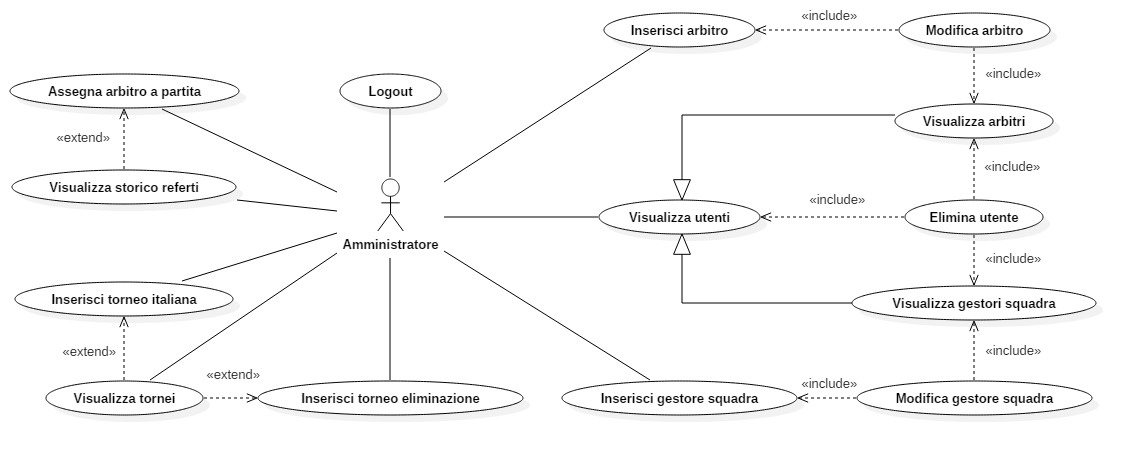
\includegraphics[width=1\textwidth]
	{immagini/uc-amministratore}
	
	\caption{Casi d'uso dell'attore amministratore}
\end{figure}

%
% Caso d'uso: Logout
%
\subsection{Caso d'uso: Logout}

\subsubsection*{Descrizione}
Questa funzionalità permette all'amministratore di uscire dalla sua pagina e di iniziare a navigare come utente pubblico.
Il pulsante di Logout è presente in ogni pagina dell'applicazione web, in alto a destra.

\subsubsection*{Attori coinvolti}
Amministratore, partecipazione attiva dell'attore verso il caso d'uso medesimo.

\subsubsection*{Pre-condizioni}
È richiesto l'accesso al sistema tramite la funzionalità di login.

\subsubsection*{Post-condizioni}
Termina la sessione di accesso al sistema in qualità di amministratore.

\subsubsection*{Flusso principale}

\begin{enumerate}
	
	\item
	L'amministratore seleziona nella pagina in cui si trova il pulsante di Logout;
	
	\item
	Il sistema scollega l'amministratore dalle pagine a lui riservate;
	
	\item
	Il sistema redireziona l'amministratore nella schermata di login e da quel momento può navigare come utente pubblico.
	
\end{enumerate}

\subsubsection*{Flussi alternativi}
Nel caso di operazione non riuscita si notifica all'amministratore il tipo di errore che si è verificato.

\subsection*{Diagramma delle attività}
Il diagramma delle attività per il caso d'uso ``Logout'' è illustrato nella figura \vref{ad-logout}.


%
% Caso d'uso: Inserisci arbitro
%
\subsection{Caso d'uso: Inserisci arbitro}
\label{uc-inserisci-arbitro}

\subsubsection*{Descrizione}
Questa funzionalità permette all'amministratore di creare un nuovo utente di tipo arbitro.

\subsubsection*{Attori coinvolti}
Amministratore, partecipazione attiva dell'attore verso il caso d'uso medesimo.
L'amministratore interagisce direttamente con il sistema compilando i campi richiesti.

Arbitro, partecipazione non attiva in quanto si procede solo alla creazione di tale attore.

\subsubsection*{Pre-condizioni}
È richiesto l'accesso al sistema come amministratore, tramite la funzionalità di login, in quanto solo lui ha il privilegio di poter inserire un arbitro.

\subsubsection*{Post-condizioni}
Viene aggiornato lo stato sul database con l'inserimento di un nuovo arbitro. L'arbitro è associato all'amministratore.

\subsubsection*{Flusso principale}

\begin{enumerate}
	
	\item
	L'amministratore seleziona la voce ``Nuovo Arbitro'' nella propria home page oppure seleziona la voce ``Inserisci Nuovo Arbitro''nella pagina di visualizzazione degli utenti;
	
	\item
	L'amministratore inserisce per l'arbitro i seguenti dati: nome, cognome, email, password, indirizzo, telefono, data di nascita, nazionalità, foto e carriera;
	
	\item
	L'amministratore invia la richiesta di creazione del nuovo utente al sistema;
	
	\item
	In caso di email già presente nel database viene notificato con un messaggio l'indisponibilità della email inserita invitando l'amministratore ad inserire una nuova mail;
	
	\item
	Se tutti i dati sono stati inseriti correttamente, il sistema inserisce l'arbitro nel database;
	
	\item
	Il sistema visualizza i dati dell'arbitro appena inserito dando la possibilità all'amministratore di modificare i dati.
	
\end{enumerate}

\subsubsection*{Flussi alternativi}
Nel caso di inserimento errato dei dati da parte dell'amministratore o di operazione non riuscita, si notifica all'amministratore il tipo di errore che si è verificato.


%
% Caso d'uso: Modifica arbitro
%
\subsection{Caso d'uso: Modifica arbitro}

\subsubsection*{Descrizione}
Questa funzionalità permette all'amministratore di modificare i dati di un arbitro presente nel database.

\subsubsection*{Attori coinvolti}
Amministratore, partecipazione attiva dell'attore verso il caso d'uso medesimo.
L'amministratore interagisce direttamente con il sistema modificando alcuni dei campi richiesti.

Arbitro, partecipazione non attiva in quanto si procede solo alla modifica di tale attore.

\subsubsection*{Pre-condizioni}
È richiesto l'accesso al sistema come amministratore, tramite la funzionalità di login, in quanto solo lui ha il privilegio di poter modificare un arbitro.

\subsubsection*{Post-condizioni}
Viene aggiornato lo stato sul database con la modifica di un arbitro.

\subsubsection*{Flusso principale}

\begin{enumerate}
	
	\item
	L'amministratore seleziona la voce ``Utenti'' nella pagina in cui si trova;
	
	\item
	L'amministratore seleziona la voce ``Arbitro'' per visualizzare gli utenti di tipo arbitro;
	
	\item
	L'amministratore seleziona la voce ``Modifica'', per l'arbitro che desidera modificare, nella lista degli arbitri;
	
	\item
	L'amministratore può modificare per l'arbitro i seguenti dati: nome, cognome, email, password, indirizzo, telefono, data di nascita, nazionalità, foto e carriera;
	
	\item
	L'amministratore invia la richiesta di modifica dell'arbitro al sistema;
	
	\item
	In caso di modifica dell'email con l'inserimento di una email già presente nel database, viene notificato, con un messaggio, l'indisponibilità della email inserita invitando l'amministratore ad inserire una nuova mail;
	
	\item
	Se tutti i dati sono stati inseriti correttamente, il sistema modifica l'arbitro nel database;
	
	\item
	Il sistema visualizza i dati dell'arbitro appena modificato dando la possibilità all'amministratore di effettuare ulteriori modifiche.
	
\end{enumerate}

\subsubsection*{Flussi alternativi}
Nel caso di operazione non riuscita, si notifica all'amministratore il tipo di errore che si è verificato.

\subsubsection*{Punti di inclusione}
Si può accedere a questo caso d'uso quando si effettua l'inserimento di un nuovo arbitro, vedi caso d'uso \vref{uc-inserisci-arbitro}, oppure quando si visualizza la lista di gli arbitri creati dall'amministratore, vedi caso d'uso \vref{uc-visualizza-arbitri}.


%
% Caso d'uso: Visualizza arbitri
%
\subsection{Caso d'uso: Visualizza arbitri}
\label{uc-visualizza-arbitri}

\subsubsection*{Descrizione}
Questa funzionalità permette di visualizzare la lista di tutti gli arbitri creati dall'amministratore.

\subsubsection*{Attori coinvolti}
Amministratore, partecipazione attiva dell'attore verso il caso d'uso medesimo.

\subsubsection*{Pre-condizioni}
È richiesto l'accesso al sistema come amministratore, tramite la funzionalità di login, in quanto solo lui ha il privilegio di poter visualizzare i propri arbitri.

\subsubsection*{Post-condizioni}
Nessuna post-condizione in quanto la visualizzazione degli arbitri non contribuisce a cambiare lo stato del sistema.

\subsubsection*{Flusso principale}

\begin{enumerate}
	
	\item
	L'amministratore seleziona la voce ``Utenti'' nella pagina in cui si trova;
	
	\item
	L'amministratore selezione la voce ``Arbitro'' nella pagina utenti;
	
	\item
	Il sistema visualizza tutti gli arbitri in ordine alfabetico mostrandone: id, cognome, nome, email, indirizzo e telefono. Il sistema, inoltre, visualizza per ogni utente un pulsante per eliminare l'utente e un pulsante per modificare l'utente.
	
\end{enumerate}

\subsubsection*{Flussi alternativi}
Nel caso di operazione non riuscita, si notifica all'amministratore il tipo di errore che si è verificato.


%
% Caso d'uso: Visualizza utenti
%
\subsection{Caso d'uso: Visualizza utenti}
\label{uc-visualizza-utenti}

\subsubsection*{Descrizione}
Questa funzionalità permette di visualizzare la lista di tutti gli utenti creati dall'amministratore.

\subsubsection*{Attori coinvolti}
Amministratore, partecipazione attiva dell'attore verso il caso d'uso medesimo.

\subsubsection*{Pre-condizioni}
È richiesto l'accesso al sistema come amministratore, tramite la funzionalità di login, in quanto solo lui ha il privilegio di poter visualizzare i propri utenti.

\subsubsection*{Post-condizioni}
Nessuna post-condizione in quanto la visualizzazione degli utenti non contribuisce a cambiare lo stato del sistema.

\subsubsection*{Flusso principale}

\begin{enumerate}
	
	\item
	L'amministratore seleziona la voce ``Utenti'' nella pagina in cui si trova;
	
	\item
	Il sistema visualizza tutti gli utenti in ordine alfabetico mostrandone: id, cognome, nome, email, indirizzo e telefono. Il sistema, inoltre, visualizza per ogni utente un pulsante per eliminare l'utente.
	
\end{enumerate}

\subsubsection*{Flussi alternativi}
Nel caso di operazione non riuscita, si notifica all'amministratore il tipo di errore che si è verificato.

\subsubsection*{Punti di specializzazione}
Questo caso d'uso si può specializzare in Visualizza Arbitri, vedi caso d'uso \vref{uc-visualizza-arbitri}, oppure Visualizza gestori squadra, vedi caso d'uso \vref{uc-visualizza-gestori-squadra}.


%
% Caso d'uso: Visualizza gestori squadra
%
\subsection{Caso d'uso: Visualizza gestori squadra}
\label{uc-visualizza-gestori-squadra}

\subsubsection*{Descrizione}
Questa funzionalità permette di visualizzare la lista di tutti i gestori di squadra creati dall'amministratore.

\subsubsection*{Attori coinvolti}
Amministratore, partecipazione attiva dell'attore verso il caso d'uso medesimo.

\subsubsection*{Pre-condizioni}
È richiesto l'accesso al sistema come amministratore, tramite la funzionalità di login, in quanto solo lui ha il privilegio di poter visualizzare i propri gestori di squadra.

\subsubsection*{Post-condizioni}
Nessuna post-condizione in quanto la visualizzazione dei gestori di squadra non contribuisce a cambiare lo stato del sistema.

\subsubsection*{Flusso principale}

\begin{enumerate}
	
	\item
	L'amministratore seleziona la voce ``Utenti'' nella pagina in cui si trova;
	
	\item
	L'amministratore selezione la voce ``Gestore'' nella pagina utenti;
	
	\item
	Il sistema visualizza tutti gli gestore di squadra in ordine alfabetico mostrandone: id, cognome, nome, email, indirizzo e telefono. Il sistema, inoltre, visualizza per ogni utente un pulsante per eliminare l'utente e un pulsante per modificare l'utente.
	
\end{enumerate}

\subsubsection*{Flussi alternativi}
Nel caso di operazione non riuscita, si notifica all'amministratore il tipo di errore che si è verificato.


%
% Caso d'uso: Inserisci gestore squadra
%
\subsection{Caso d'uso: Inserisci gestore squadra}
\label{uc-inserisci-gestore-squadra}

\subsubsection*{Descrizione}
Questa funzionalità permette all'amministratore di creare un nuovo utente di tipo gestore squadra.

\subsubsection*{Attori coinvolti}
Amministratore, partecipazione attiva dell'attore verso il caso d'uso medesimo.
L'amministratore interagisce direttamente con il sistema compilando i campi richiesti.

Gestore squadra, partecipazione non attiva in quanto si procede solo alla creazione di tale attore.

\subsubsection*{Pre-condizioni}
È richiesto l'accesso al sistema come amministratore, tramite la funzionalità di login, in quanto solo lui ha il privilegio di poter inserire un gestore di una squadra.

\subsubsection*{Post-condizioni}
Viene aggiornato lo stato sul database con l'inserimento di un nuovo gestore di squadra. Il gestore di squadra è associato all'amministratore.

\subsubsection*{Flusso principale}

\begin{enumerate}
	
	\item
	L'amministratore seleziona la voce ``Nuovo Gestore Squadra'' nella propria home page oppure seleziona la voce ``Inserisci Nuovo Gestore Squadra''nella pagina di visualizzazione degli utenti;
	
	\item
	L'amministratore inserisce per il gestore squadra i seguenti dati: nome, cognome, email, password, indirizzo, telefono e nome della squadra che andrà a gestire;
	
	\item
	L'amministratore invia la richiesta di creazione del nuovo utente al sistema;
	
	\item
	In caso di email già presente nel database viene notificato con un messaggio l'indisponibilità della email inserita invitando l'amministratore ad inserire una nuova mail;
	
	\item
	Se tutti i dati sono stati inseriti correttamente, il sistema inserisce nel database il gestore della squadra e una nuova squadra associato ad esso;
	
	\item
	Il sistema visualizza i dati del gestore appena inserito dando la possibilità all'amministratore di modificare i dati.
	
\end{enumerate}

\subsubsection*{Flussi alternativi}
Nel caso di inserimento errato dei dati da parte dell'amministratore o di operazione non riuscita, si notifica all'amministratore il tipo di errore che si è verificato.


%
% Caso d'uso: Modifica gestore squadra
%
\subsection{Caso d'uso: Modifica gestore squadra}

\subsubsection*{Descrizione}
Questa funzionalità permette all'amministratore di modificare i dati di un gestore squadra presente nel database.

\subsubsection*{Attori coinvolti}
Amministratore, partecipazione attiva dell'attore verso il caso d'uso medesimo.
L'amministratore interagisce direttamente con il sistema modificando alcuni dei campi richiesti.

Gestore squadra, partecipazione non attiva in quanto si procede solo alla modifica di tale attore.

\subsubsection*{Pre-condizioni}
È richiesto l'accesso al sistema come amministratore, tramite la funzionalità di login, in quanto solo lui ha il privilegio di poter modificare un gestore di una squadra.

\subsubsection*{Post-condizioni}
Viene aggiornato lo stato sul database con la modifica di un  gestore di una squadra.

\subsubsection*{Flusso principale}

\begin{enumerate}
	
	\item
	L'amministratore seleziona la voce ``Utenti'' nella pagina in cui si trova;
	
	\item
	L'amministratore seleziona la voce ``Gestore'' per visualizzare gli utenti di tipo gestore squadra;
	
	\item
	L'amministratore seleziona la voce ``Modifica'', per il gestore squadra che desidera modificare, nella lista degli arbitri;
	
	\item
	L'amministratore può modificare per l'arbitro i seguenti dati: nome, cognome, email, password, indirizzo, telefono e squadra;
	
	\item
	L'amministratore invia la richiesta di modifica dell'arbitro al sistema;
	
	\item
	In caso di modifica dell'email con l'inserimento di una email già presente nel database, viene notificato, con un messaggio, l'indisponibilità della email inserita invitando l'amministratore ad inserire una nuova mail;
	
	\item
	Se tutti i dati sono stati inseriti correttamente, il sistema modifica il gestore squadra nel database;
	
	\item
	Il sistema visualizza i dati del gestore squadra appena modificato dando la possibilità all'amministratore di effettuare ulteriori modifiche.
	
\end{enumerate}

\subsubsection*{Flussi alternativi}
Nel caso di operazione non riuscita, si notifica all'amministratore il tipo di errore che si è verificato.

\subsubsection*{Punti di inclusione}
Si può accedere a questo caso d'uso quando si effettua l'inserimento di un nuovo gestore squadra, vedi caso d'uso \vref{uc-inserisci-gestore-squadra}, oppure quando si visualizza la lista di tutti i gestori squadra creati dall'amministratore, vedi caso d'uso \vref{uc-visualizza-gestori-squadra}.


%
% Caso d'uso: Elimina utente
%
\subsection{Caso d'uso: Elimina utente}

\subsubsection*{Descrizione}
Questa funzionalità permette all'amministratore di eliminare un utente registrato e, conseguentemente, di invalidare l'accesso delle credenziali dell'utente eliminato all'applicazione web.

\subsubsection*{Attori coinvolti}
Amministratore, partecipazione attiva dell'attore verso il caso d'uso medesimo.
L'amministratore interagisce direttamente con il sistema eliminando l'utente selezionato.

\subsubsection*{Pre-condizioni}
È richiesto l'accesso al sistema come amministratore, tramite la funzionalità di login, in quanto solo lui ha il privilegio di poter eliminare i propri utenti.

\subsubsection*{Post-condizioni}
Viene aggiornato lo stato sul database con l'eliminazione dell'utente selezionato.

\subsubsection*{Flusso principale}

\begin{enumerate}
	
	\item
	L'amministratore seleziona la voce ``Elimina'', per l'utente che desidera eliminare, nella lista degli utenti;
	
	\item
	Il sistema chiede la conferma di esecuzione dell'operazione;
	
	\item
	Se l'amministratore conferma l'operazione l'utente viene eliminato altrimenti l'operazione viene annullata.
	
\end{enumerate}

\subsubsection*{Flussi alternativi}
Nel caso di operazione non riuscita, si notifica all'amministratore il tipo di errore che si è verificato.

\subsubsection*{Punti di inclusione}
Si può accedere a questo caso d'uso quando si effettua la visualizzazione di tutti gli utenti, vedi caso d'uso \vref{uc-visualizza-utenti}, quando si visualizza la lista di tutti gli arbitri creati dall'amministratore, vedi caso d'uso \vref{uc-visualizza-arbitri}, quando si visualizza la lista di tutti i gestori squadra creati dall'amministratore, vedi caso d'uso \vref{uc-visualizza-gestori-squadra}.


%
% Caso d'uso: Inserisci torneo eliminazione
%
\subsection{Caso d'uso: Inserisci torneo eliminazione}

\subsubsection*{Descrizione}
Questa funzionalità permette all'amministratore di creare un nuovo torneo ad eliminazione diretta.

\subsubsection*{Attori coinvolti}
Amministratore, partecipazione attiva dell'attore verso il caso d'uso medesimo.
L'amministratore interagisce direttamente con il sistema compilando i campi richiesti.

\subsubsection*{Pre-condizioni}
È richiesto l'accesso al sistema come amministratore, tramite la funzionalità di login, in quanto solo lui ha il privilegio di poter creare un torneo ad eliminazione.

\subsubsection*{Post-condizioni}
Viene aggiornato lo stato sul database con l'inserimento di un nuovo torneo ad eliminazione.

\subsubsection*{Flusso principale}

\begin{enumerate}
	
	\item
	L'amministratore seleziona la voce ``Nuovo Torneo Eliminazione'' nella propria home page o nella pagina di visualizzazione dei tornei;
	
	\item
	Il sistema restituisce la pagina web dove l'amministratore inserirà: il nome del torneo, il numero di squadre partecipanti e una descrizione relativa al torneo;
	
	\item
	L'amministratore prosegue con la creazione cliccando sul pulsante ``Continua'';
	
	\item
	Il sistema controlla che tutti i dati siano stati inseriti correttamente e visualizza la lista delle squadre complete presenti sul sistema (una squadra è completa quando il gestore di squadra ha compilato tutti i campi relativi alla propria squadra altrimenti la squadra non può partecipare ai tornei).
	
	\item
	L'amministratore seleziona le squadre da iscrivere al torneo;
	
	\item
	Il sistema controlla che sia stato inserito il giusto numero di squadre;
	
	\item
	Il sistema chiede la conferma all'amministratore e, in caso affermativo, il sistema crea il torneo;
	
	\item
	Il sistema notifica il successo dell'operazione all'amministratore visualizzando il tabellone degli incontri.
	
\end{enumerate}

\subsubsection*{Flussi alternativi}
Nel caso di inserimento errato dei dati da parte dell'amministratore o di operazione non riuscita, si notifica all'amministratore il tipo di errore che si è verificato.

\subsubsection*{Punti di estensione}
Si può accedere a questo caso d'uso quando si effettua la visualizzazione della lista di tutti i tornei creati dall'amministratore, vedi caso d'uso \vref{uc-visualizza-tornei}, ma si tratta di un accesso opzionale.


%
% Caso d'uso: Visualizza tornei
%
\subsection{Caso d'uso: Visualizza tornei}
\label{uc-visualizza-tornei}

\subsubsection*{Descrizione}
Questa funzionalità permette all'amministratore di vedere i tornei da lui creati e di monitorarne l'andamento.

\subsubsection*{Attori coinvolti}
Amministratore, partecipazione attiva dell'attore verso il caso d'uso medesimo.
L'amministratore richiede la visualizzazione delle pagine.

\subsubsection*{Pre-condizioni}
È richiesto l'accesso al sistema come amministratore, tramite la funzionalità di login.

\subsubsection*{Post-condizioni}
Nessuna post-condizione in quanto la visualizzazione dei tornei non contribuisce a cambiare lo stato del sistema.

\subsubsection*{Flusso principale}

\begin{enumerate}
	
	\item
	L'amministratore seleziona la voce ``Tornei'' nella pagina in cui si trova;
	
	\item
	Il sistema invia la pagina richiesta con la lista dei tornei creati dall'amministratore.
	
\end{enumerate}

\subsubsection*{Flussi alternativi}
Nel caso di operazione non riuscita, si notifica all'amministratore il tipo di errore che si è verificato.


%
% Caso d'uso: Inserisci torneo italiana
%
\subsection{Caso d'uso: Inserisci torneo italiana}

\subsubsection*{Descrizione}
Questa funzionalità permette all'amministratore di creare un nuovo torneo all'italiana.

\subsubsection*{Attori coinvolti}
Amministratore, partecipazione attiva dell'attore verso il caso d'uso medesimo.
L'amministratore interagisce direttamente con il sistema compilando i campi richiesti.

\subsubsection*{Pre-condizioni}
È richiesto l'accesso al sistema come amministratore, tramite la funzionalità di login, in quanto solo lui ha il privilegio di poter creare un torneo all'italiana.

\subsubsection*{Post-condizioni}
Viene aggiornato lo stato sul database con l'inserimento di un nuovo torneo all'italiana.

\subsubsection*{Flusso principale}

\begin{enumerate}
	
	\item
	L'amministratore seleziona la voce ``Nuovo Torneo Italiana'' nella propria home page o nella pagina di visualizzazione dei tornei;
	
	\item
	Il sistema restituisce la pagina web dove l'amministratore inserirà: il nome del torneo, il numero di squadre partecipanti e una descrizione relativa al torneo;
	
	\item
	L'amministratore prosegue con la creazione cliccando sul pulsante ``Continua'';
	
	\item
	Il sistema controlla che tutti i dati siano stati inseriti correttamente e visualizza la lista delle squadre complete presenti sul sistema (una squadra è completa quando il gestore di squadra ha compilato tutti i campi relativi alla propria squadra altrimenti la squadra non può partecipare ai tornei).
	
	\item
	L'amministratore seleziona le squadre da iscrivere al torneo;
	
	\item
	Il sistema controlla che sia stato inserito il giusto numero di squadre;
	
	\item
	Il sistema chiede la conferma all'amministratore e, in caso affermativo, il sistema crea il torneo;
	
	\item
	Il sistema notifica il successo dell'operazione all'amministratore visualizzando il tabellone delle varie giornate.
	
\end{enumerate}

\subsubsection*{Flussi alternativi}
Nel caso di inserimento errato dei dati da parte dell'amministratore o di operazione non riuscita, si notifica all'amministratore il tipo di errore che si è verificato.

\subsubsection*{Punti di estensione}
Si può accedere a questo caso d'uso quando si effettua la visualizzazione della lista di tutti i tornei creati dall'amministratore, vedi caso d'uso \vref{uc-visualizza-tornei}, ma si tratta di un accesso opzionale.

\subsection*{Diagramma delle attività}
Il diagramma delle attività per il caso d'uso ``Inserisci torneo all'italiana'' è illustrato nella figura \vref{ad-creazione-torneo-italiana}.


%
% Figura: diagramma delle attività relativo alla creazione del torneo all'italiana
%
\begin{figure}[h]
	\centering
	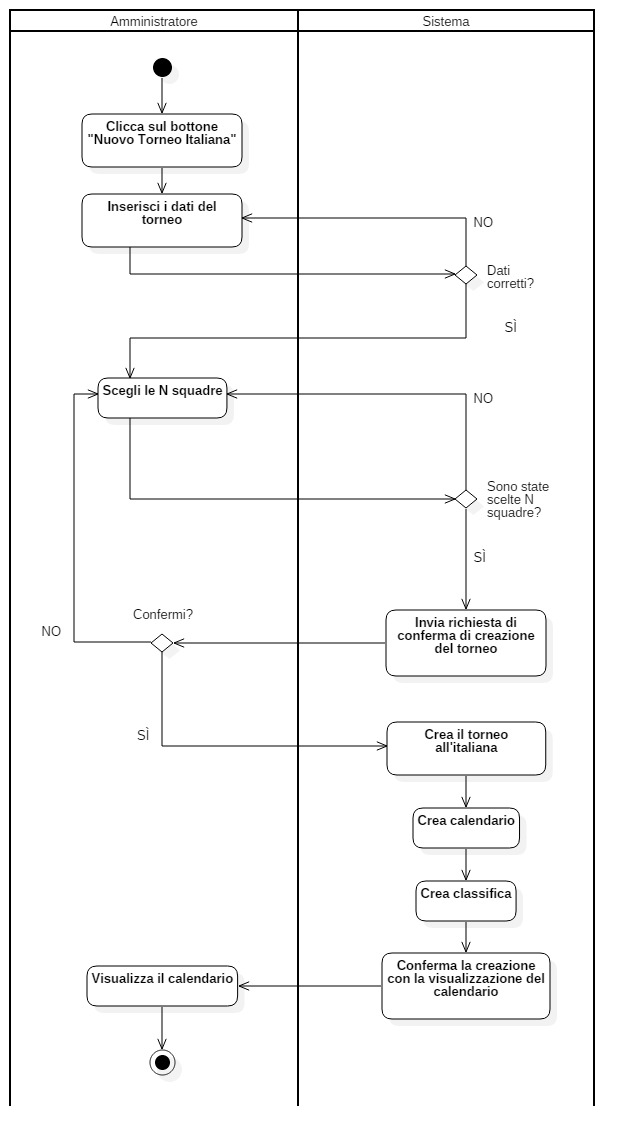
\includegraphics[width=0.8\textwidth]
	{immagini/ad-creazione-torneo-italiana}
	
	\caption{Diagramma delle attività della creazione di un torneo all'italiana}
	\label{ad-creazione-torneo-italiana}
\end{figure}


%
% Caso d'uso: Visualizza storico referti
%
\subsection{Caso d'uso: Visualizza storico referti}
\label{uc-visualizza-storico-referti}

\subsubsection*{Descrizione}
Questa funzionalità permette all'amministratore di vedere tutti i referti che l'amministratore ha assegnato ai rispettivi arbitri.

\subsubsection*{Attori coinvolti}
Amministratore, partecipazione attiva dell'attore verso il caso d'uso medesimo.
L'amministratore richiede la visualizzazione delle pagine.

\subsubsection*{Pre-condizioni}
È richiesto l'accesso al sistema come amministratore, tramite la funzionalità di login, in quanto solo lui ha il privilegio di poter visualizzare tale pagina.

\subsubsection*{Post-condizioni}
Nessuna post-condizione in quanto la visualizzazione dello storico dei referti non contribuisce a cambiare lo stato del sistema.

\subsubsection*{Flusso principale}

\begin{enumerate}
	
	\item
	L'amministratore seleziona la voce ``Referti'' nella pagina in cui si trova;
	
	\item
	Il sistema invia la pagina richiesta con la lista dei referti e dei rispettivi arbitri a cui sono stati assegnati dall'amministratore.
	
\end{enumerate}

\subsubsection*{Flussi alternativi}
Nel caso di operazione non riuscita, si notifica all'amministratore il tipo di errore che si è verificato.


%
% Caso d'uso: Assegna arbitro a partita
%
\subsection{Caso d'uso: Assegna arbitro a partita}

\subsubsection*{Descrizione}
Questa funzionalità permette all'amministratore di assegnare un arbitro ad una partita di un determinato torneo, associando all'arbitro un referto che dovrà essere compilato al termine della partita.

\subsubsection*{Attori coinvolti}
Amministratore, partecipazione attiva dell'attore verso il caso d'uso medesimo.
L'amministratore interagisce direttamente con il sistema compilando i campi richiesti.

Arbitro, partecipazione non attiva in quanto si procede solo all'assegnazione di un referto a tale attore.

\subsubsection*{Pre-condizioni}
È richiesto l'accesso al sistema come amministratore, tramite la funzionalità di login, in quanto solo lui ha il privilegio di poter assegnare un arbitro ad una partita di un torneo.

\subsubsection*{Post-condizioni}
Viene aggiornato lo stato sul database con l'inserimento di un nuovo referto e con l'associazione del referto appena creato con un arbitro presente nel database.

\subsubsection*{Flusso principale}

\begin{enumerate}
	
	\item
	L'amministratore seleziona la voce ``Assegna arbitro'' nella propria home page oppure seleziona la voce ``Assegna Arbitro a Partita'' nella pagina di visualizzazione dei referti;
	
	\item
	L'amministratore seleziona il torneo;
	
	\item
	L'amministratore seleziona la giornata/fase del torneo;
	
	\item
	Se per tale fase/giornata sono disponibili incontri non ancora assegnati, l'amministratore può selezionare la partita altrimenti il sistema visualizza un messaggio di indisponibilità delle partite;
	
	\item
	L'amministratore sceglie un arbitro ed inserisce per la partita: data, orario e luogo;
	
	\item
	L'amministratore preme il pulsante di ``Conferma assegnazione''.
	
	\item
	Il sistema chiede conferma all'amministratore dell'assegnazione dell'arbitro alla partita. Se l'amministratore acconsente il sistema elabora i dati, altrimenti non avviene alcuna operazione e permette all'amministratore di modificare i dati inseriti;
	
	\item
	Il sistema modifica lo stato del database aggiornando i dati della partita e inserendo un nuovo referto;
	
	\item
	Il sistema notifica l'amministratore l'esito positivo dell'operazione, visualizzando il referto appena inserito nello storico dei referti. 
	
\end{enumerate}

\subsubsection*{Flussi alternativi}
Nel caso di operazione non riuscita, si notifica all'amministratore il tipo di errore che si è verificato.

\subsubsection*{Punti di estensione}
Si può accedere a questo caso d'uso quando si effettua la visualizzazione della lista dello storico dei referti creati dall'amministratore, vedi caso d'uso \vref{uc-visualizza-storico-referti}, ma si tratta di un accesso opzionale.   % modello dei casi d'uso: amministratore
% !TEX encoding = UTF-8
% !TEX TS-program = pdflatex
% !TEX root = ../Tesi.tex
% !TEX spellcheck = it-IT

\clearpage

\section{Attore gestore della squadra}
%
% Figura: casi d'uso dell'attore gestore della squadra
%
\begin{figure}[h]
	\centering
	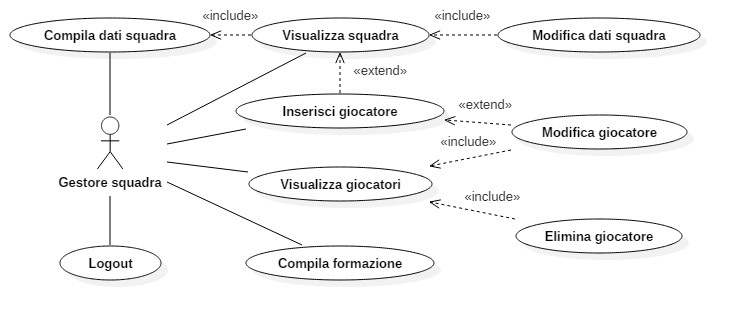
\includegraphics[width=0.8\textwidth]
	{immagini/uc-gestore-squadra}
	
	\caption{Casi d'uso dell'attore gestore della squadra}
\end{figure}


%
% Caso d'uso: Logout
%
\subsection{Caso d'uso: Logout}

\subsubsection*{Descrizione}
Questa funzionalità permette al gestore della squadra di uscire dalla sua pagina e di iniziare a navigare come utente pubblico.
Il pulsante di Logout è presente in ogni pagina dell'applicazione web, in alto a destra.

\subsubsection*{Attori coinvolti}
Gestore della squadra, partecipazione attiva dell'attore verso il caso d'uso medesimo.

\subsubsection*{Pre-condizioni}
È richiesto l'accesso al sistema tramite la funzionalità di login.

\subsubsection*{Post-condizioni}
Termina la sessione di accesso al sistema in qualità di gestore della squadra.

\subsubsection*{Flusso principale}

\begin{enumerate}
	
	\item
	Il gestore della squadra seleziona nella pagina in cui si trova il pulsante di Logout;
	
	\item
	Il sistema scollega l'amministratore dalle pagine a lui riservate;
	
	\item
	Il sistema redireziona il gestore della squadra nella schermata di login e da quel momento può navigare come utente pubblico.
	
\end{enumerate}

\subsubsection*{Flussi alternativi}
Nel caso di operazione non riuscita si notifica all'amministratore il tipo di errore che si è verificato.

\subsection*{Diagramma delle attività}
Il diagramma delle attività per il caso d'uso ``Logout'' è illustrato nella figura \vref{ad-logout}.

%
% Caso d'uso: Inserisci giocatore
%
\subsection{Caso d'uso: Inserisci giocatore}
\label{uc-inserisci-giocatore}

\subsubsection*{Descrizione}
Questa funzionalità permette al gestore squadra di inserire nella rosa della propria squadra un nuovo giocatore.

\subsubsection*{Attori coinvolti}
Gestore squadra, partecipazione attiva dell'attore verso il caso d'uso medesimo.
Il gestore squadra interagisce direttamente con il sistema compilando i campi richiesti.

\subsubsection*{Pre-condizioni}
È richiesto l'accesso al sistema come gestore squadra, tramite la funzionalità di login, in quanto solo lui può inserire un nuovo giocatore nella sua squadra. Il gestore squadra può inserire al massimo 36 giocatori.

\subsubsection*{Post-condizioni}
Viene aggiornato lo stato sul database con l'inserimento di un nuovo giocatore.

\subsubsection*{Flusso principale}

\begin{enumerate}
	
	\item
	Il gestore squadra seleziona la voce ``Nuovo Giocatore'' nella propria home page oppure seleziona la voce ``Inserisci Nuovo Giocatore'' nella pagina di visualizzazione della squadra oppure seleziona la voce ``Inserisci Nuovo Giocatore'' nella pagina di visualizzazione dei giocatori;
	
	\item
	Il gestore squadra inserisce per il giocatore i seguenti dati: nome, cognome, data di nascita, nazionalità, numero di maglia, ruolo, foto e descrizione;
	
	\item
	Il gestore squadra invia la richiesta di creazione del nuovo giocatore al sistema;
	
	\item
	Il sistema controlla che il gestore della squadra abbia inserito correttamente tutti i dati. Se i dati sono corretti il sistema crea un nuovo giocatore;
	
	\item
	Il sistema visualizza i dati del giocatore appena inserito dando la possibilità al gestore della squadra di modificarli;
	
\end{enumerate}

\subsubsection*{Flussi alternativi}
Nel caso di operazione non riuscita, si notifica al gestore della squadra il tipo di errore che si è verificato.


%
% Caso d'uso: Elimina giocatore
%
\subsection{Caso d'uso: Elimina giocatore}

\subsubsection*{Descrizione}
Questa funzionalità permette al gestore della squadra di eliminare un giocatore dalla rosa della squadra che gestisce.

\subsubsection*{Attori coinvolti}
Gestore squadra, partecipazione attiva dell'attore verso il caso d'uso medesimo.
Il gestore squadra interagisce direttamente con il sistema eliminando il giocatore selezionato.

\subsubsection*{Pre-condizioni}
È richiesto l'accesso al sistema come gestore squadra, tramite la funzionalità di login, in quanto solo lui ha il privilegio di poter eliminare i propri giocatori.

\subsubsection*{Post-condizioni}
Viene aggiornato lo stato sul database con l'eliminazione del giocatore selezionato.

\subsubsection*{Flusso principale}

\begin{enumerate}
	
	\item
	Il gestore della squadra seleziona la voce ``Elimina'', per il giocatore che desidera eliminare, nella lista dei giocatori;
	
	\item
	Il sistema chiede la conferma di esecuzione dell'operazione;
	
	\item
	Se il gestore della squadra conferma l'operazione il giocatore viene eliminato altrimenti l'operazione viene annullata.
	
\end{enumerate}

\subsubsection*{Flussi alternativi}
Nel caso di operazione non riuscita, si notifica al gestore della squadra il tipo di errore che si è verificato.

\subsubsection*{Punti di inclusione}
Si può accedere a questo caso d'uso quando si effettua la visualizzazione di tutti i giocatori, vedi caso d'uso \vref{uc-visualizza-giocatori}.


%
% Caso d'uso: Visualizza giocatori
%
\subsection{Caso d'uso: Visualizza giocatori}
\label{uc-visualizza-giocatori}

\subsubsection*{Descrizione}
Questa funzionalità permette di visualizzare la lista di tutti gli i giocatori creati da un gestore di una squadra.

\subsubsection*{Attori coinvolti}
Gestore squadra, partecipazione attiva dell'attore verso il caso d'uso medesimo.

\subsubsection*{Pre-condizioni}
È richiesto l'accesso al sistema come gestore squadra, tramite la funzionalità di login.

\subsubsection*{Post-condizioni}
Nessuna post-condizione in quanto la visualizzazione dei giocatori non contribuisce a cambiare lo stato del sistema.

\subsubsection*{Flusso principale}

\begin{enumerate}
	
	\item
	Il gestore della squadra seleziona la voce ``Giocatori'' nella pagina in cui si trova;
	
	\item
	Il sistema visualizza tutti i giocatori in ordine alfabetico mostrandone: foto, nome, cognome, numero maglia e ruolo. Il sistema, inoltre, visualizza per ogni utente un pulsante per eliminare l'utente e il pulsante per modificare l'utente.
	
\end{enumerate}

\subsubsection*{Flussi alternativi}
Nel caso di operazione non riuscita, si notifica al gestore della squadra il tipo di errore che si è verificato.


%
% Caso d'uso: Visualizza squadra
%
\subsection{Caso d'uso: Visualizza squadra}
\label{uc-visualizza-squadra}

\subsubsection*{Descrizione}
Questa funzionalità permette al gestore della squadre di visualizzare la propria squadra.

\subsubsection*{Attori coinvolti}
Gestore squadra, partecipazione attiva dell'attore verso il caso d'uso medesimo.

\subsubsection*{Pre-condizioni}
È richiesto l'accesso al sistema come gestore squadra, tramite la funzionalità di login.

\subsubsection*{Post-condizioni}
Nessuna post-condizione in quanto la visualizzazione della squadra non contribuisce a cambiare lo stato del sistema.

\subsubsection*{Flusso principale}

\begin{enumerate}
	
	\item
	Il gestore della squadra seleziona la voce ``Visualizza Squadra'' nella sua home page oppure seleziona nella pagina in cui si trova la voce ``Squadra'';
	
	\item
	Il sistema visualizza i dati della squadra mostrandone: nome, logo, immagine della squadra, sede, descrizione, nome dello sponsor e logo dello sponsor.
	
\end{enumerate}

\subsubsection*{Flussi alternativi}
Nel caso il gestore della squadra non abbia compilato i dati della squadra si attiva il caso d'uso Compila squadra, vedi caso d'uso \vref{uc-compila-squadra}.

Nel caso di operazione non riuscita, si notifica al gestore della squadra il tipo di errore che si è verificato.


%
% Caso d'uso: Modifica squadra
%
\subsection{Caso d'uso: Modifica squadra}
\label{uc-modifica-squadra}

\subsubsection*{Descrizione}
Questa funzionalità permette al gestore squadra di modificare i dati della propria squadra.

\subsubsection*{Attori coinvolti}
Gestore squadra, partecipazione attiva dell'attore verso il caso d'uso medesimo.
Il gestore squadra interagisce direttamente con il sistema compilando i campi richiesti.

\subsubsection*{Pre-condizioni}
È richiesto l'accesso al sistema come gestore squadra, tramite la funzionalità di login, in quanto solo lui può modificare i dati della sua squadra.

\subsubsection*{Post-condizioni}
Viene aggiornato lo stato sul database con l'aggiornamento dei dati di una squadra.

\subsubsection*{Flusso principale}

\begin{enumerate}
	
	\item
	Il gestore della squadra seleziona la voce ``Modifica'' nella pagina di visualizzazione della squadra oppure seleziona la voce ``Inserisci Nuovo Giocatore'' nella pagina di visualizzazione dei giocatori;
	
	\item
	Il gestore della squadra inserisce per la squadra i seguenti dati: nome, sede, foto della squadra, logo della squadra, nome dello sponsor, immagine dello sponsor e descrizione della squadra;
	
	\item
	Il gestore della squadra seleziona la voce ``Conferma Modifiche'';
	
	\item
	Il sistema controlla che il gestore della squadra abbia inserito correttamente tutti i dati. Se i dati sono corretti il sistema invia una richiesta di conferma dei dati inseriti al gestore della squadra;
	
	\item
	Se il gestore della squadra conferma la modifica allora il sistema visualizza la pagina della squadra con i dati aggiornati;
	
\end{enumerate}

\subsubsection*{Flussi alternativi}
Nel caso di operazione non riuscita, si notifica al gestore della squadra il tipo di errore che si è verificato.

\subsection*{Diagramma delle attività}
Il diagramma delle attività per il caso d'uso ``Modifica squadra'' è illustrato nella figura \vref{ad-modifica-squadra}.


%
% Figura: diagramma delle attività relativo alla creazione del torneo all'italiana
%
\begin{figure}[h]
	\centering
	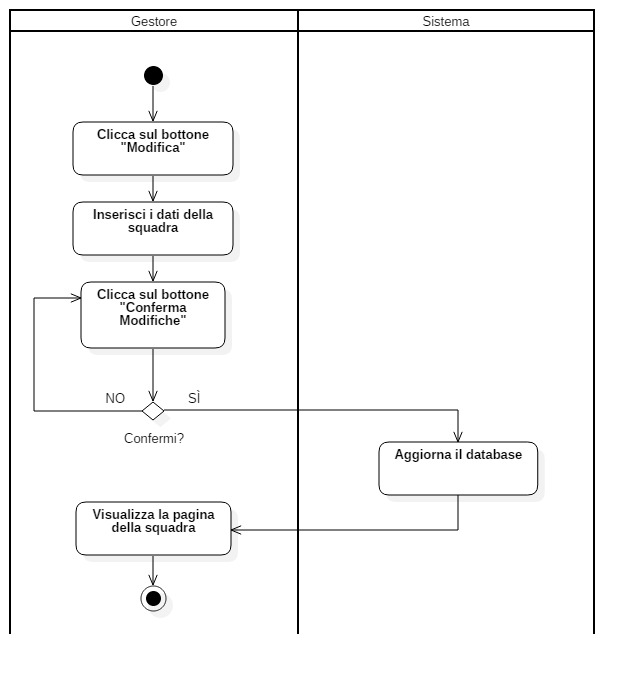
\includegraphics[width=0.8\textwidth]
	{immagini/ad-modifica-squadra}
	
	\caption{Diagramma delle attività di modifica della squadra}
	\label{ad-modifica-squadra}
\end{figure}


%
% Caso d'uso: Compila formazione
%
\subsection{Caso d'uso: Compila formazione}

\subsubsection*{Descrizione}
Questa funzionalità permette al gestore squadra di scegliere i giocatori che faranno parte ad una formazione in una determinata partita.

\subsubsection*{Attori coinvolti}
Gestore squadra, partecipazione attiva dell'attore verso il caso d'uso medesimo.

Il gestore squadra interagisce direttamente con il sistema scegliendo 11 giocatori titolari e 7 riserve.

\subsubsection*{Pre-condizioni}
È richiesto l'accesso al sistema come gestore squadra, tramite la funzionalità di login, in quanto solo lui può compilare la formazione per una partita.

\subsubsection*{Post-condizioni}
Viene aggiornato lo stato sul database con l'inserimento della formazione scelta dal gestore della squadra.

\subsubsection*{Flusso principale}

\begin{enumerate}
	
	\item
	Il gestore della squadra seleziona la voce ``Nuova Formazione'' nella propria home page oppure seleziona la voce ``Formazioni'' nella pagina di visualizzazione dei giocatori;
	
	\item
	Il sistema visualizza la lista di tutte le partite a cui il gestore deve fornire la formazione dove per ogni partita vengono visualizzate le seguenti informazioni: id del referto, nome del torneo, le due squadre sfidanti e la data della partita. Il sistema, inoltre, visualizza per ogni partita un pulsante per compilare la formazione della squadra per la partita corrispondente;
	
	\item
	Il gestore della squadra seleziona una partita;
	
	\item
	Il sistema visualizza la lista di tutti i giocatori che fanno parte della squadra con a lato la possibilità di scegliere se far giocare un giocatore come titolare o come riserva;
	
	\item
	Il gestore della squadra sceglie 11 giocatori titolari e 7 giocatori riserve;
	
	\item
	Il gestore seleziona la voce ``Conferma Formazione'';
	
	\item
	Il sistema controlla che il gestore della squadra abbia selezionato correttamente i giocatori. Se i giocatori sono stati selezionati correttamente il sistema invia una richiesta di conferma della formazione inserita al gestore della squadra altrimenti invia una notifica dell'errore commesso al gestore della squadra;
	
	\item
	Se il gestore della squadra conferma la formazione allora il sistema aggiorna il database inserendo la formazione appena compilata e visualizza la lista di tutte le partite rimanenti a cui il gestore deve fornire la formazione;
	
\end{enumerate}

\subsubsection*{Flussi alternativi}
Nel caso di operazione non riuscita, si notifica al gestore della squadra il tipo di errore che si è verificato.   % modello dei casi d'uso: gestore squadra
% !TEX encoding = UTF-8
% !TEX TS-program = pdflatex
% !TEX root = ../Tesi.tex
% !TEX spellcheck = it-IT

\clearpage

\section{Attore arbitro}
%
% Figura: casi d'uso dell'attore arbitro
%
\begin{figure}[h]
	\centering
	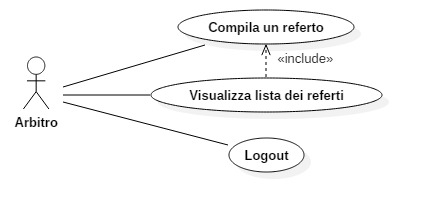
\includegraphics[width=0.7\textwidth]
	{immagini/uc-arbitro}
	
	\caption{Casi d'uso dell'attore arbitro}
\end{figure}


%
% Caso d'uso: Logout
%
\subsection{Caso d'uso: Logout}

\subsubsection*{Descrizione}
Questa funzionalità permette all'arbitro di uscire dalla sua pagina e di iniziare a navigare come utente pubblico.
Il pulsante di Logout è presente in ogni pagina dell'applicazione web, in alto a destra.

\subsubsection*{Attori coinvolti}
Arbitro, partecipazione attiva dell'attore verso il caso d'uso medesimo.

\subsubsection*{Pre-condizioni}
È richiesto l'accesso al sistema tramite la funzionalità di login.

\subsubsection*{Post-condizioni}
Termina la sessione di accesso al sistema in qualità di arbitro.

\subsubsection*{Flusso principale}

\begin{enumerate}
	
	\item
	L'arbitro seleziona nella pagina in cui si trova il pulsante di Logout;
	
	\item
	Il sistema scollega l'arbitro dalle pagine a lui riservate;
	
	\item
	Il sistema redireziona l'arbitro nella schermata di login e da quel momento può navigare come utente pubblico.
	
\end{enumerate}

\subsubsection*{Flussi alternativi}
Nel caso di operazione non riuscita si notifica all'arbitro il tipo di errore che si è verificato.

\subsection*{Diagramma delle attività}
Il diagramma delle attività per il caso d'uso ``Logout'' è illustrato nella figura \vref{ad-logout}.

%
% Caso d'uso: Visualizza lista dei referti
%
\subsection{Caso d'uso: Visualizza lista dei referti}

\subsubsection*{Descrizione}
Questa funzionalità permette all'arbitro di vedere tutti i referti che deve compilare o che ha già compilato.

\subsubsection*{Attori coinvolti}
Arbitro, partecipazione attiva dell'attore verso il caso d'uso medesimo.

\subsubsection*{Pre-condizioni}
È richiesto l'accesso al sistema come arbitro, tramite la funzionalità di login, in quanto solo lui ha il privilegio di poter visualizzare tale pagina.

\subsubsection*{Post-condizioni}
Nessuna post-condizione in quanto la visualizzazione dello dei referti non contribuisce a cambiare lo stato del sistema.

\subsubsection*{Flusso principale}

\begin{enumerate}
	
	\item
	L'arbitro seleziona la voce ``Nuovo Referto'' nella propria home page oppure seleziona la voce ``Referti'' nella pagina in cui si trova;
	
	\item
	Il sistema visualizza tutti i referti in ordine di id mostrandone: id del referto, nome del torneo, squadre sfidanti e data della partita. Il sistema, inoltre, visualizza per ogni referto un pulsante per compilarlo oppure visualizza ``Compilato'' se il referto è già stato compilato. 
	
\end{enumerate}

\subsubsection*{Flussi alternativi}
Nel caso di operazione non riuscita, si notifica all'arbitro il tipo di errore che si è verificato.


%
% Caso d'uso: Compila referto
%
\subsection{Caso d'uso: Compila referto}

\subsubsection*{Descrizione}
Questa funzionalità permette all'arbitro di compilare un referto che gli è stato assegnato relativo ad una partita.

\subsubsection*{Attori coinvolti}
Arbitro, partecipazione attiva dell'attore verso il caso d'uso medesimo.

Amministratore, partecipazione non attiva dell'attore verso il caso d'uso medesimo in quanto l'amministratore è responsabile solo della creazione della partita che l'arbitro dovrà dirigere.

Gestore squadra, partecipazione non attiva dell'attore verso il caso d'uso medesimo in quanto il gestore della squadra ha fornito la formazione della squadra per la partita a cui riferisce il referto.

\subsubsection*{Pre-condizioni}
È richiesto l'accesso al sistema come arbitro, tramite la funzionalità di login, in quanto solo lui ha il privilegio di poter compilare il referto di una partita. È richiesto che l'arbitro sia stato assegnato alla partita dall'amministratore. È necessario che entrambe le squadre abbiano fornito la formazione per la partita a cui fa riferimento il referto.

\subsubsection*{Post-condizioni}
Viene aggiornato lo stato sul database con l'aggiornamento del referto e viene aggiornata la classifica delle due squadre che hanno disputato l'incontro. In caso di torneo ad eliminazione diretta si provvede a qualificare al turno successivo la squadra che ha vinto.

\subsubsection*{Flusso principale}

\begin{enumerate}
	
	\item
	L'arbitro seleziona la voce ``Compila'' nella pagina di visualizzazione dei referti;
	
	\item
	Il sistema visualizza la pagina per l'inserimento dell'orario di inizio e l'orario di fine della partita;
	
	\item
	L'arbitro inserisce gli orari effettivi di inizio e fine della partita e successivamente seleziona la voce ``Conferma Orari'';
	
	\item
	Il sistema controlla i dati inseriti e se sono corretti visualizza le due formazioni con i giocatori di entrambe le squadre. Per ogni giocatore il sistema visualizza: foto del giocatore, numero maglia, nome e cognome del giocatore, campo per inserire il numero di goal effettuati e campo per inserire il numero di ammonizioni. Il sistema, inoltre, visualizza il numero di autogol effettuati per ciascuna squadra;
	
	\item
	L'arbitro inserisce i campi richiesti e conferma l'inserimento selezionando la voce ``Conferma'';
	
	\item
	Il sistema chiede conferma all'arbitro della compilazione del referto della partita. Se l'arbitro acconsente il sistema elabora i dati, altrimenti non avviene alcuna operazione e permette all'arbitro di modificare i dati inseriti;
	
\end{enumerate}

\subsubsection*{Flussi alternativi}
Nel caso di operazione non riuscita, si notifica all'arbitro il tipo di errore che si è verificato.

\subsection*{Diagramma delle attività}
Il diagramma delle attività per il caso d'uso ``Compila referto'' è illustrato nella figura \vref{ad-referto}.


%
% Figura: diagramma delle attività relativo alla compilazione di un referto
%
\begin{figure}[h]
	\centering
	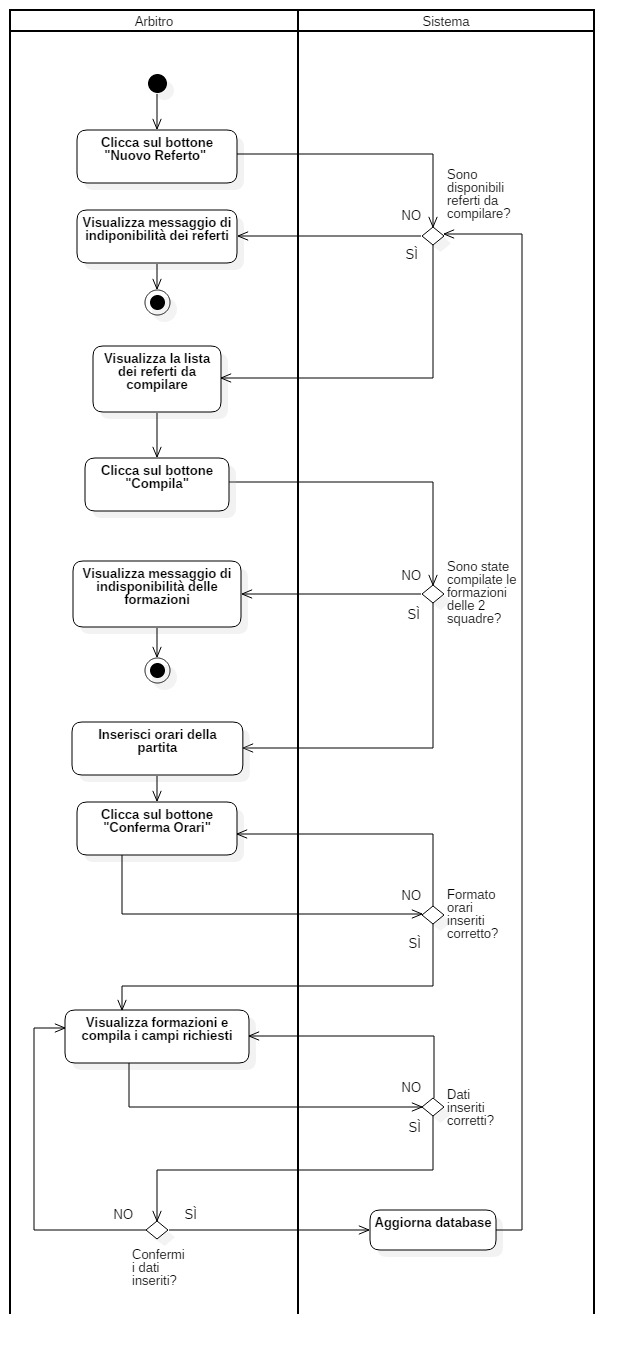
\includegraphics[width=0.8\textwidth]
	{immagini/ad-referto}
	
	\caption{Diagramma delle attività della compilazione di un referto}
	\label{ad-referto}
\end{figure}


%
% Figura: diagramma delle attività relativo al logout di un utente
%
\begin{figure}
	\centering
	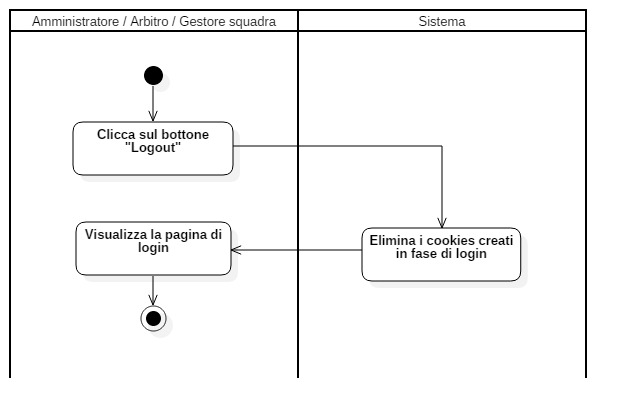
\includegraphics[width=0.8\textwidth]
	{immagini/ad-logout}
	
	\caption{Diagramma delle attività del logout di un utente}
	\label{ad-logout}
\end{figure}   % modello dei casi d'uso: arbitro
% !TEX encoding = UTF-8
% !TEX TS-program = pdflatex
% !TEX root = ../Tesi.tex
% !TEX spellcheck = it-IT

\clearpage

\section{Attore utente pubblico}
%
% Figura: casi d'uso dell'attore utente pubblico
%
\begin{figure}[h]
	\centering
	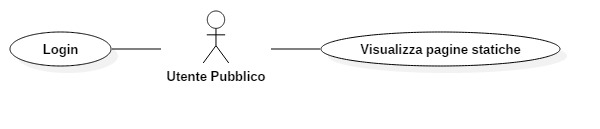
\includegraphics[width=0.9\textwidth]
	{immagini/uc-utente-pubblico}
	
	\caption{Casi d'uso dell'attore utente pubblico}
\end{figure}


%
% Caso d'uso: Visualizza pagine statiche
%
\subsection{Caso d'uso: Visualizza pagine statiche}

	\subsubsection*{Descrizione}
	Questa funzionalità permette all'utente pubblico di visualizzare tutte le pagine richieste con contenuto non dinamico.
	
	\subsubsection*{Attori coinvolti}
	Utente pubblico, partecipazione attiva, richiedendo la visualizzazione delle pagine.
	
	\subsubsection*{Pre-condizioni}
	Nessuna precondizione, in quanto non serve uno stato particolare per visualizzare una pagina statica.
	
	\subsubsection*{Post-condizioni}
	Nessuna postcondizione, in quanto la visualizzazione di una pagina statica non altera lo stato dell'applicazione.
	
	\subsubsection*{Flusso principale}
	
	\begin{enumerate}
		
		\item
		Richiesta di qualsiasi pagina che abbia contenuto statico da parte dell'utente pubblico
		
		\item
		Risposta del server con la pagina statica richiesta da parte dell'utente pubblico;
		
	\end{enumerate}
	
	\subsubsection*{Flussi alternativi}
	Non presenti.

%
% Caso d'uso: Effettua login
%
\subsection{Caso d'uso: Effettua login}

	\subsubsection*{Descrizione}
	Questa funzionalità permette all'utente pubblico di farsi riconoscere dal sistema, accedendo quindi alle funzionalità che sono a lui riservate.
	
	\subsubsection*{Attori coinvolti}
	Utente pubblico, partecipazione attiva dell'attore che passa da Utente Pubblico ad Amministratore o Gestore squadra o Arbitro.
	
	\subsubsection*{Pre-condizioni}
	Compilazione del modulo di login.
	
	\subsubsection*{Post-condizioni}
	L'utente passa da attore Utente Pubblico ad Amministratore o Gestore squadra o Arbitro.
	
	\subsubsection*{Flusso principale}
	
	\begin{enumerate}
		
		\item
		L'utente pubblico seleziona la voce ``Login'' nella pagina in cui si trova;
		
		\item
		L'utente pubblico compila il modulo inserendo la propria email e la propria password;
		
		\item
		L'utente pubblico seleziona la voce ``Accedi'';
		
		\item
		Il sistema effettua verifica se le informazioni inserite nel campo email sono corrette dal punto di vista sintattico inviando all'utente pubblico, in caso di errore, una notifica con l'errore riscontrato;
		
		\item
		Il sistema dopo aver ricevuto i dati il server controlla se nella base dati è presente un utente con indirizzo email e password ricevuti;
		
		\item
		Se le informazioni esistono sulla base dati l'utente pubblico viene riconosciuto dal sistema. L'utente visualizza il suo nome e cognome con un messaggio di benvenuto che lo informa della sua tipologia. L'utente selezionando la voce ``MyHome'' visualizza la propria home page e un menù con tutte le operazioni che può eseguire sul sistema.
		
	\end{enumerate}
	
	\subsubsection*{Flussi alternativi}
	Nel caso di inserimento di email e password non presenti nel database vengono notificate all'utente pubblico le possibili cause di errore.
	
	\subsection*{Diagramma delle attività}
	Il diagramma delle attività per il caso d'uso ``Effettua login'' è illustrato nella figura \vref{ad-login}.
	
	
	%
	% Figura: diagramma delle attività relativo al login di un utente
	%
	\begin{figure}[h]
		\centering
		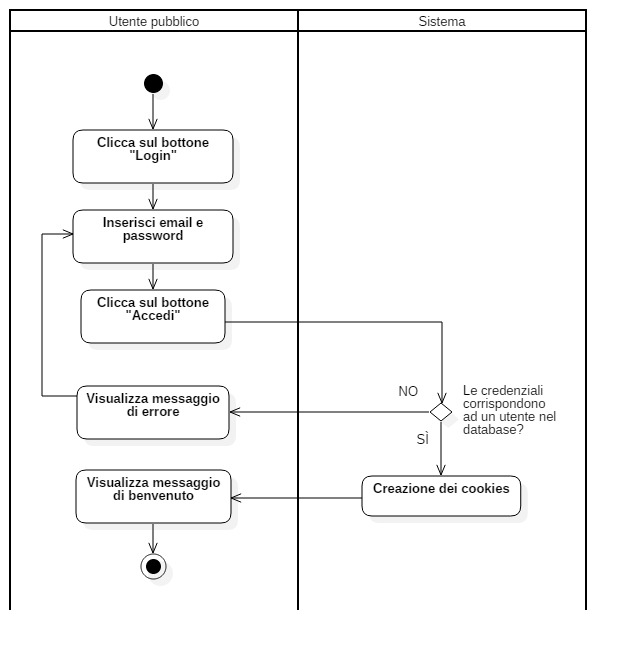
\includegraphics[width=0.8\textwidth]
		{immagini/ad-login}
		
		\caption{Diagramma delle attività del login di un utente pubblico}
		\label{ad-login}
	\end{figure}   % modello dei casi d'uso: utente pubblico
% !TEX encoding = UTF-8
% !TEX TS-program = pdflatex
% !TEX root = ../Tesi.tex
% !TEX spellcheck = it-IT

%************************************************
\chapter{Modello del dominio}
\label{cap:modello-del-dominio}
%************************************************

\section{Diagramma delle classi}
Si presenta ora il modello delle classi di dominio.

\section{Diagramma degli stati}      % modello del dominio
% !TEX encoding = UTF-8
% !TEX TS-program = pdflatex
% !TEX root = ../Tesi.tex
% !TEX spellcheck = it-IT

%************************************************
\chapter{Modello di design}
\label{cap:modello-di-design}
%************************************************

\section{Diagramma delle classi}
	Il raffinamento del modello delle classi di dominio avviene attraverso il modello di design suddividendo tutte le classi del progetto in tre categorie:
	\begin{enumerate}
		
		\item
		Classi Boundary;
		
		\item
		Classi Control;
		
		\item
		Classi Entity.
		
	\end{enumerate}
	Di seguito vengono presentate le categorie sopracitate.

	\subsection{Classi Boundary}
	Sono le classi che si interfacciano con l'utente.
	
	Le classi boundary rappresentano un punto di interfaciamento bidirezionale tra gli attori ed il sistema.
	
	Nel caso dell'applicazione web, queste sono le singole pagine JSP che in fase di compilazione vengono convertite in Servlet (classi Java che estendono la classe \texttt{HTTPServlet}).
	
	Gli attori sono: Admin (amministratore), Arbitro, Gestore (gestore di una squadra) e Guest (utente pubblico).
	
	Si procede con l'elenco delle classi Boundary:
	
	\subsubsection*{Admin:}
	
		\begin{itemize}
			\item Calendario.jsp
			\item dettagliTorneo.jsp
			\item dettagliUtente.jsp
			\item homeA.jsp
			\item newReferto.jsp
			\item newTorneo.jsp
			\item referti.jsp
			\item refertiView.jsp
			\item selezionaSquadre.jsp
			\item tornei.jsp
			\item utenti.jsp	
		\end{itemize}
	
	\subsubsection*{Arbitro:}
	
	\begin{itemize}
		\item dettagliReferto.jsp
		\item homeR.jsp
		\item myReferti.jsp
		\item referti.jsp	
	\end{itemize}
	
	\subsubsection*{Gestore:}
	
	\begin{itemize}
		\item dettagliGiocatore.jsp
		\item giocatori.jsp
		\item homeG.jsp
		\item newFormazione.jsp
		\item sceltaGiocatori.jsp
		\item squadre.jsp	
	\end{itemize}
	
	\subsubsection*{Guest:}
	
	\begin{itemize}
		\item listaGiocatori.jsp
		\item listaSquadre.jsp
		\item listaTornei.jsp
		\item vediGiocatore.jsp
		\item vediReferto.jsp
		\item vediSquadra.jsp
		\item vediTorneo.jsp	
	\end{itemize}

	\subsubsection*{Tutti gli utenti:}
	
	\begin{itemize}
		\item ErrorPage.jsp
		\item login.jsp
		\item home.jsp	
	\end{itemize}
	
	\subsection{Classi Control}
	Sono le classi che validano le interazioni dell'utente e si interfacciano con la base dati.
	
	Queste classi incapsulano la logica applicativa dei casi d'uso sopra elencati. Il compito di queste classi è quello di coordinare il lavoro svolto da istanze delle classi \emph{Boundary} ed \emph{Entity}.
	
	Nel caso dell'applicazione web, queste sono le classi della \emph{Business Logic}, i \emph{Services} associati e le classi che governano il flusso delle conversazioni.
	
	\subsubsection*{Package bflows:}
	Il package \texttt{bflows} (acronimo di \emph{BusinessFlows}) si occupa del controllo del flusso delle conversazioni.
	Le classi di questo package usano le classi del package \texttt{blogics} (acronimo di \emph{BusinessLogics}) che si occupano di mappare l'oggetto del database e di fornire i servizi interessati dalla conversazione medesima.
	Si nota che una conversazione può avere più classi \emph{Boundary} associate.
	
	\subsubsection*{Package blogics:}
	Il package \texttt{blogics} si occupa di rendere disponibili tutte le funzioni e i servizi che l'applicazione web può offrire.
	I servizi presenti in questo package non sono vincolati in alcun modo a particolari interfacce o a determinate conversazioni, ma possono essere utilizzate in più contesti.
	
	\subsubsection*{Package service:}
	Le classi contenute in questo package sono classi di servizio. Infatti si può notare che il costruttore di tali classi è privato e che tutti i metodi delle classi sono statici.
	
	In particolare si osserva nella classe \texttt{DBService.java} l'implementazione del pattern \emph{Singleton} che gestisce la connessione al database.
	
	\subparagraph{databaseservice}
	Le classi contenute in questa sottocartella della classe services, permettono di gestire la connessione al database.
	
	%
	% Figura: classi della cartella databaseservice
	%
	\begin{figure}[h]
		\centering
		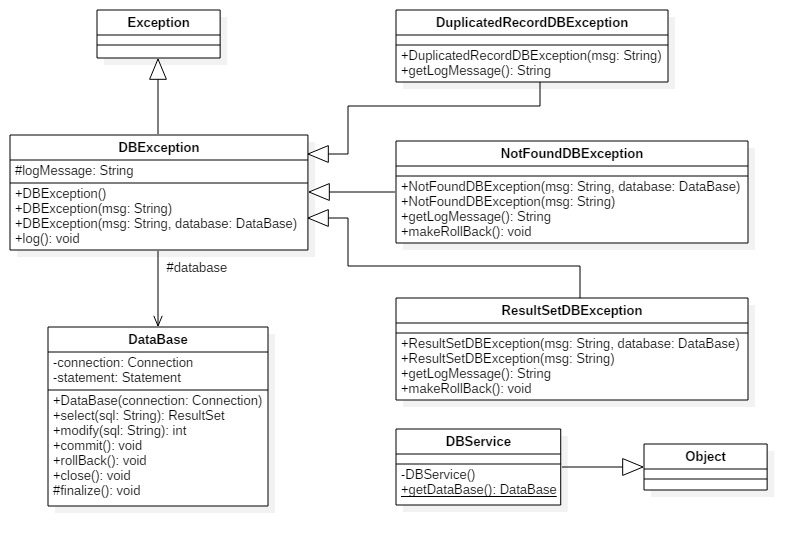
\includegraphics[width=0.4\textwidth]
		{immagini/c-databaseservice}
		
		\caption{Classi della sotto-cartella databaseservice}
	\end{figure}
	
	
	\subparagraph{errorservice}
	La classe contenuta in questa sottocartella della classe services, permette di gestire gli errori che si possono generare durante l'esecuzione dell'applicazione.
	
	%
	% Figura: classe della cartella errorservice
	%
	\begin{figure}[h]
		\centering
		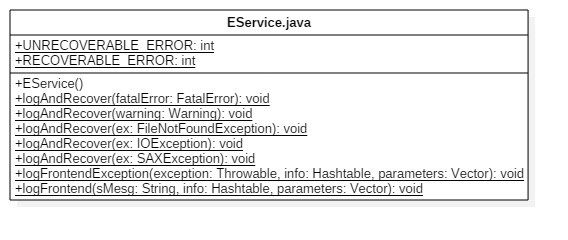
\includegraphics[width=0.4\textwidth]
		{immagini/c-errorservice}
		
		\caption{Classe della sotto-cartella errorservice}
	\end{figure}
	
	
	\subparagraph{logservice}
	Le classi contenute in questa sottocartella della classe services, permettono di scrivere i messaggi di errore in uno specifico file denominato \emph{log}.
	
	%
	% Figura: classi della cartella logservice
	%
	\begin{figure}[h]
		\centering
		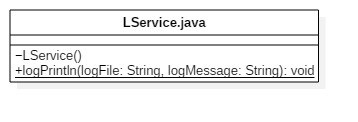
\includegraphics[width=0.4\textwidth]
		{immagini/c-logservice}
		
		\caption{Classi della sotto-cartella logservice}
	\end{figure}
	
	
	\subparagraph{sessionservice}
	La classe contenuta in questa sottocartella della classe services, permette di gestire la sessione tramite il protocollo \texttt{HTTP}.
	
	%
	% Figura: classe della cartella sessionservice
	%
	\begin{figure}[h]
		\centering
		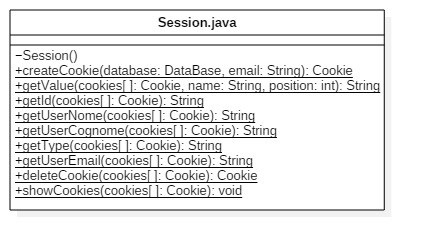
\includegraphics[width=0.4\textwidth]
		{immagini/c-sessionservice}
		
		\caption{Classe della sotto-cartella sessionservice}
	\end{figure}
	
	
	\clearpage
	
	%
	% Figura: classi del package bflows
	%
	\begin{figure}[h]
		\centering
		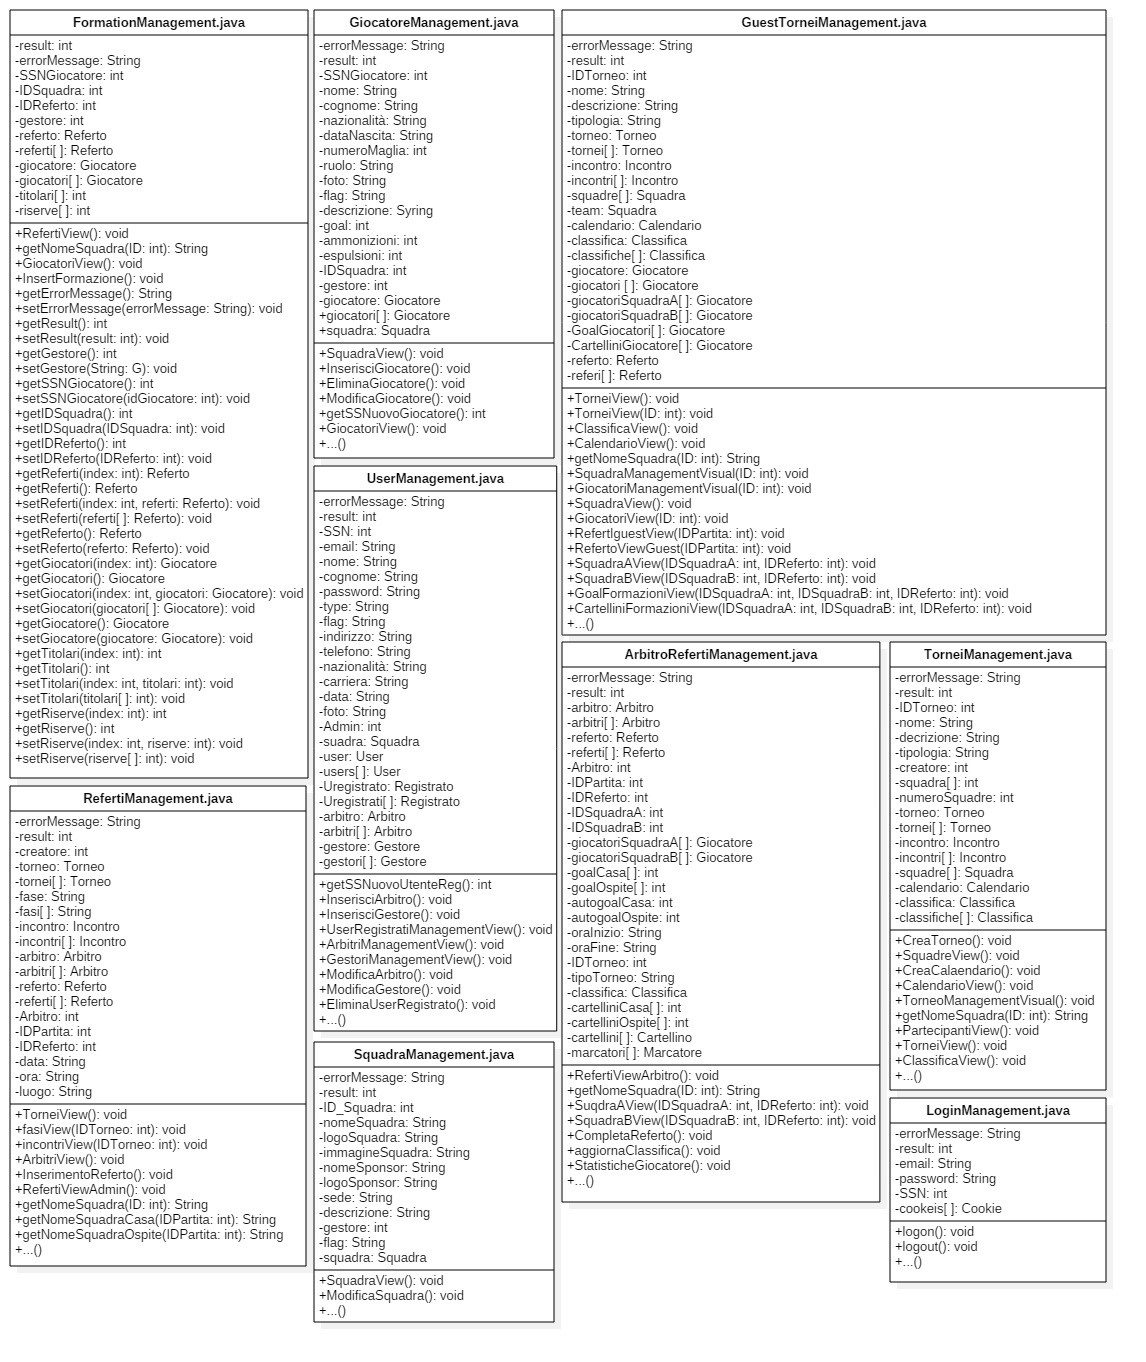
\includegraphics[width=1\textwidth]
		{immagini/c-bflows}
		
		\caption{Classi del package bflows}
	\end{figure}
	
	\subparagraph*{N.B.}
	Il simbolo $+...()$ sta indica tutti i metodi getter e setter utili per far funzionare correttamente l'applicazione. Si è scelto di non inserirli per non aggiungere ulteriore complessità ai diagrammi.
	
	\clearpage
	
	%
	% Figura: classi del package blogics
	%
	\begin{figure}[h]
		\centering
		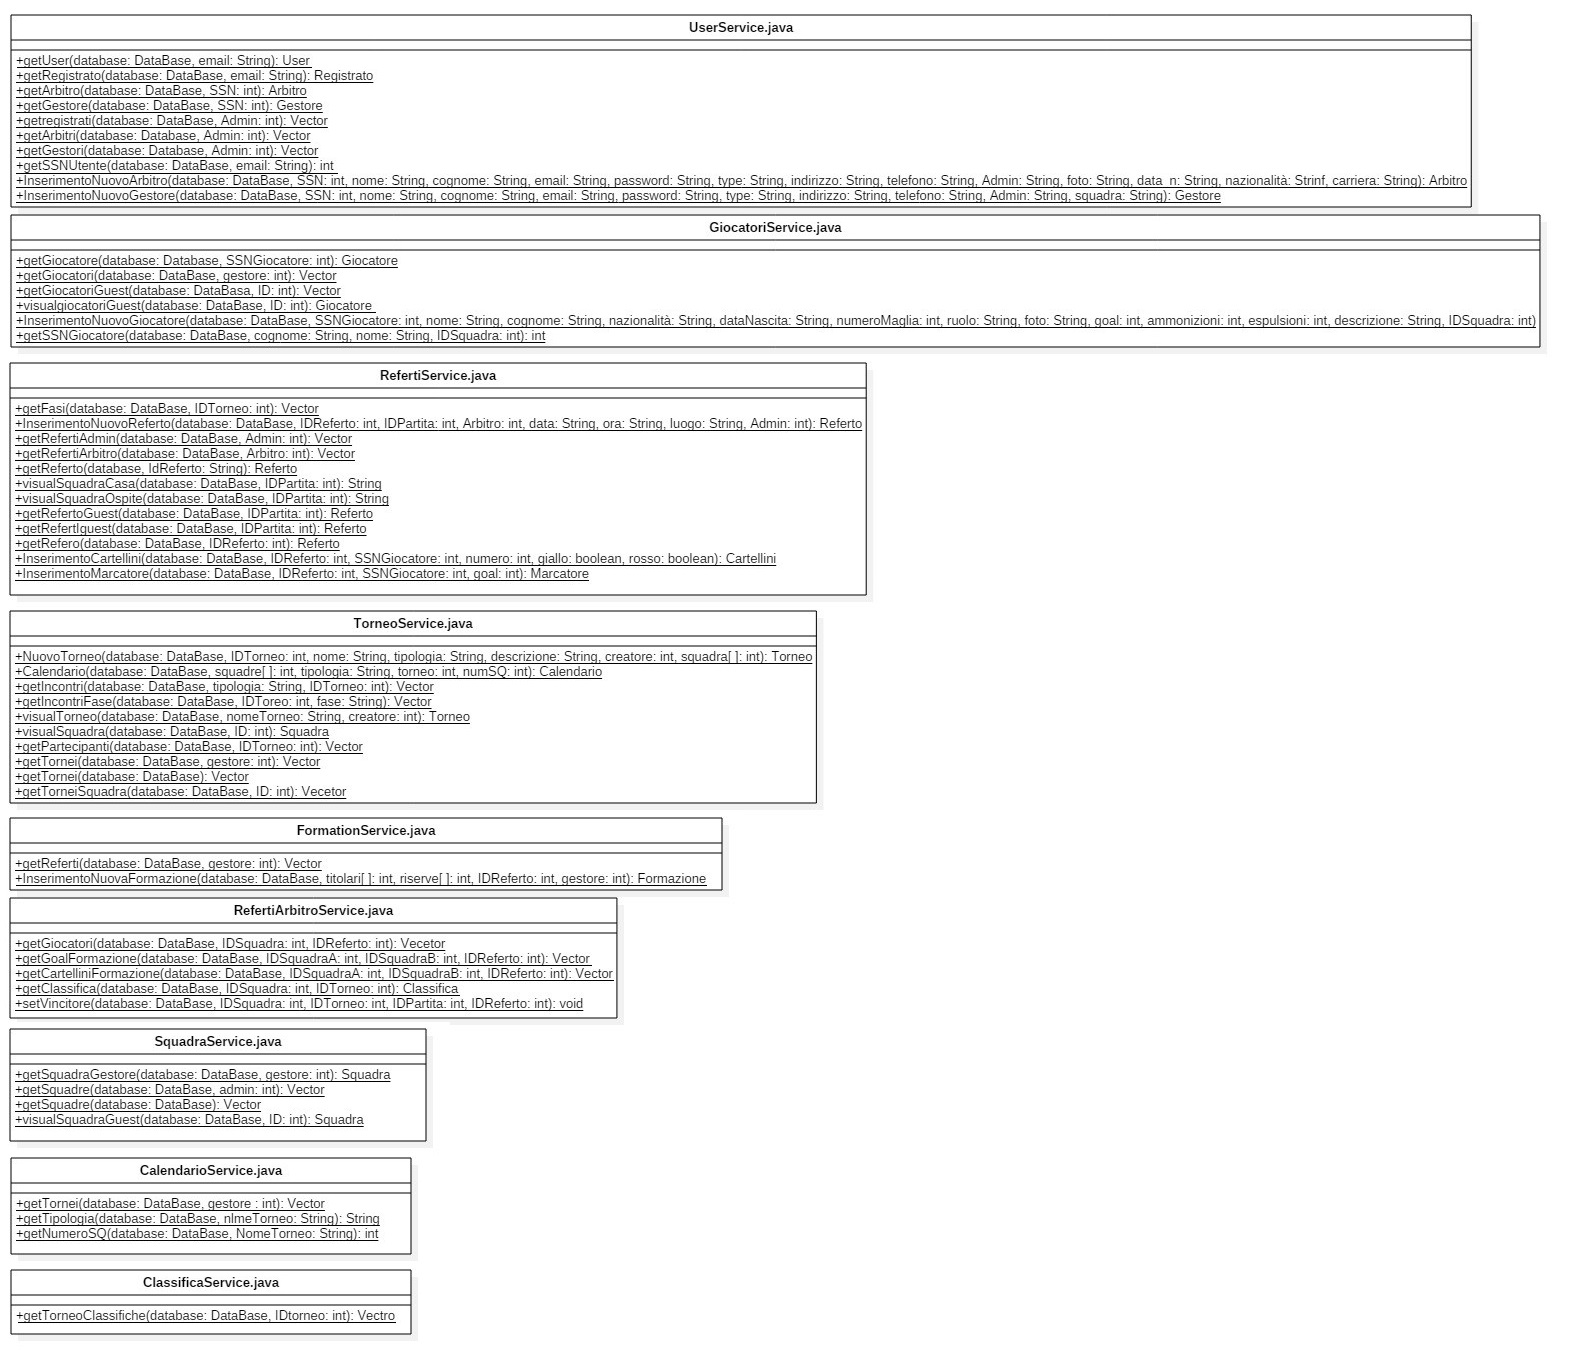
\includegraphics[width=1\textwidth]
		{immagini/c-service-blogics}
		
		\caption{Classi service del package blogics}
	\end{figure}
	
	\subsection{Classi Entity}
	\label{c4:classi-entity}
	Sono le classi che mappano la struttura della base dati.
	
	Le classi Entity modellano le informazioni gestite dal sistema e formalizzano la struttura logica dei dati, in modo da isolare i dettagli della memorizzazione dei dati e di limitare l'impatto di eventuali modifiche alla struttura del database.
	
	Nel caso dell'applicazione web, queste sono le classi della \emph{Business Logic} che implementano i metodi setter, getter e i costruttori per creare l'oggetto mediante passaggio di dati di tipo primitivo od oggetti quali \texttt{RecordSet}.
	
	La figura \vref{c-blogics} rappresenta le classi di questo tipo.
	
	%
	% Figura: classi del package blogics
	%
	\begin{figure}[h]
		\centering
		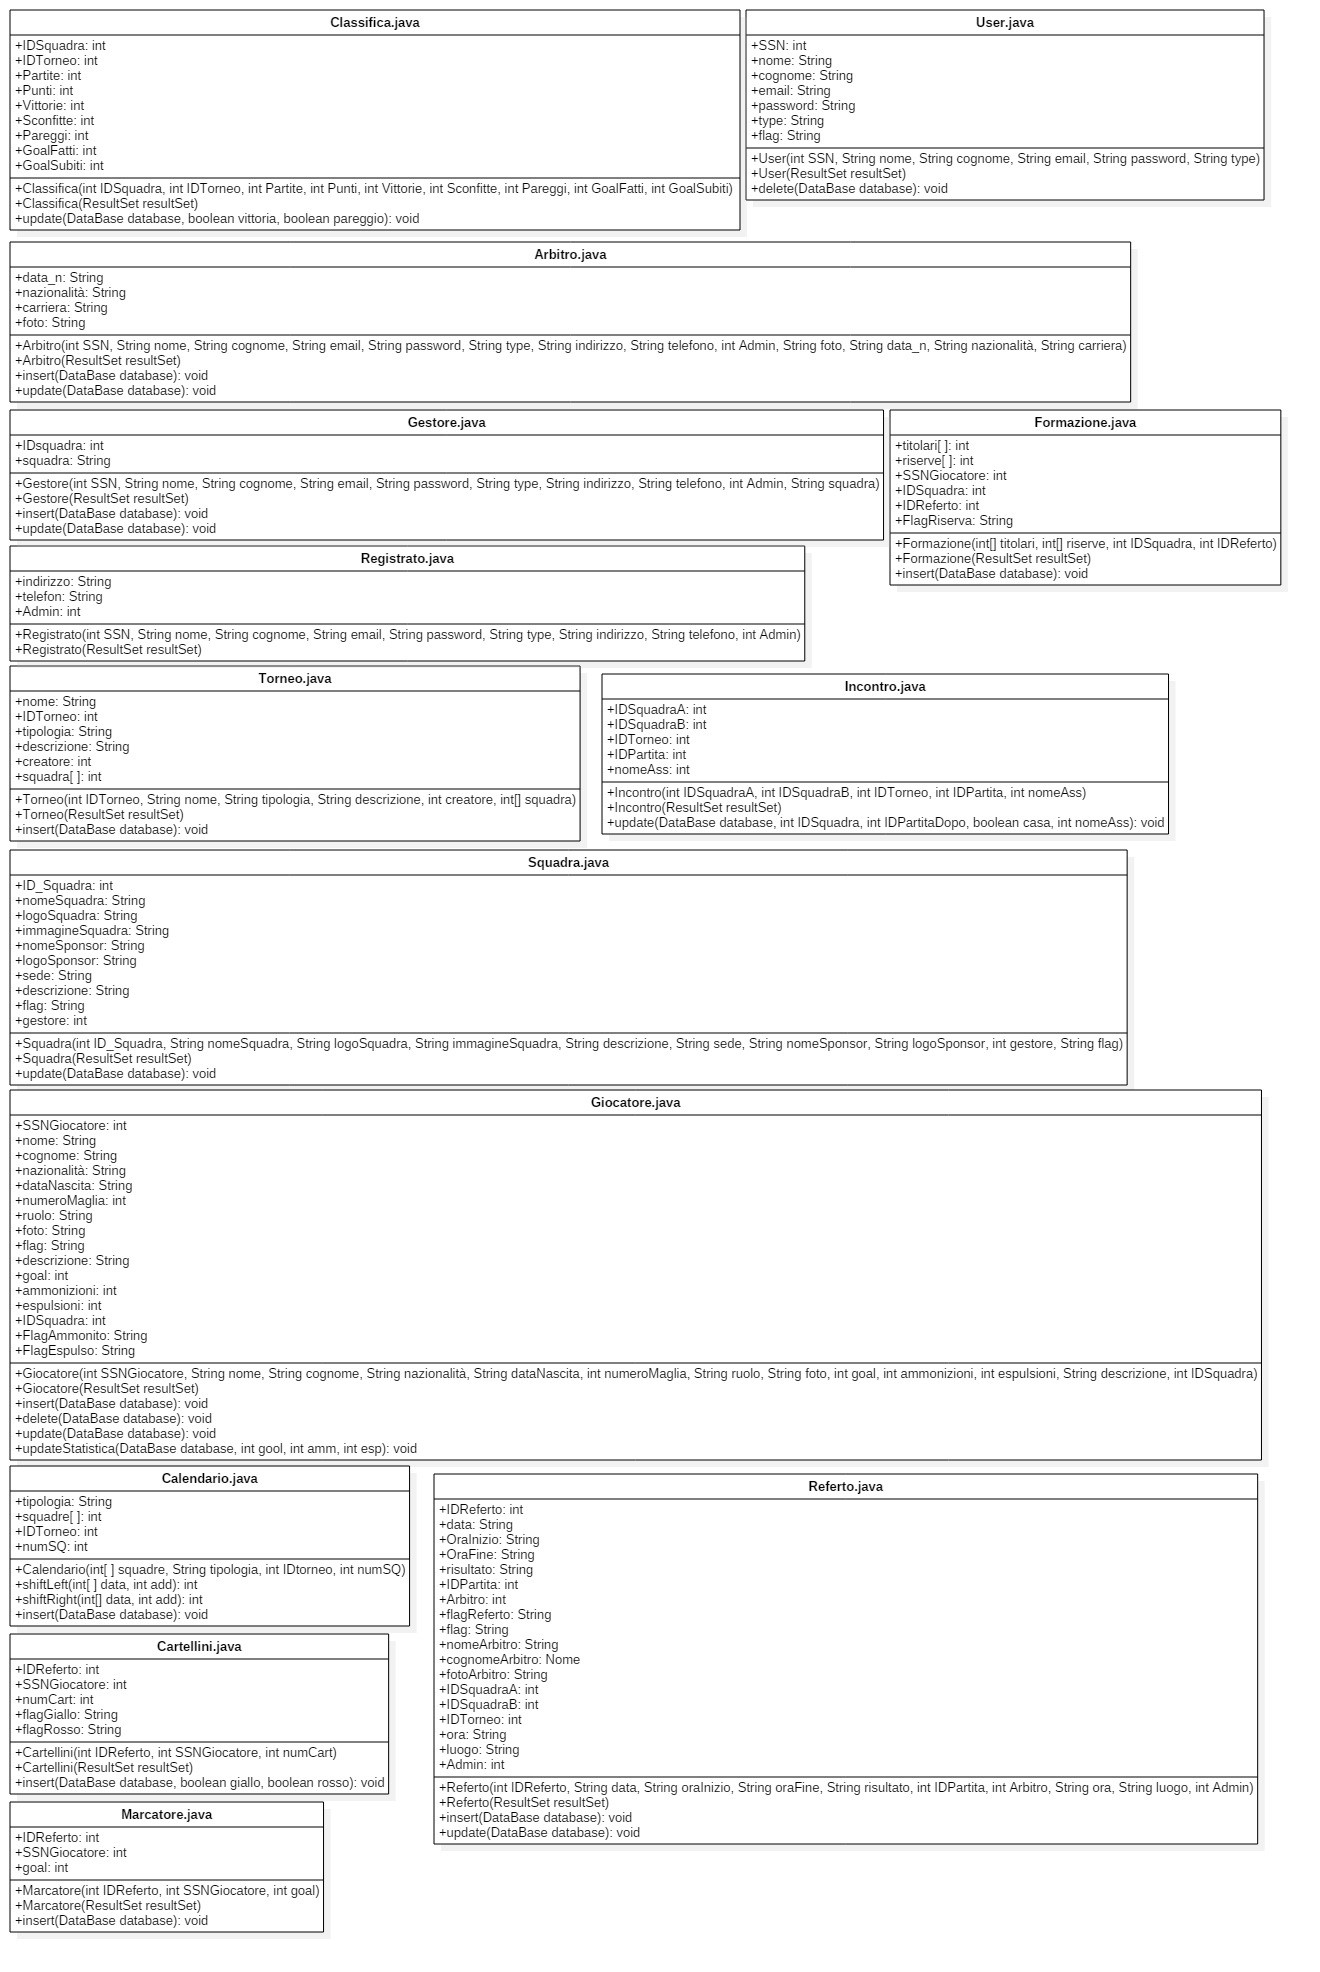
\includegraphics[width=1\textwidth]
		{immagini/c-blogics}
		
		\caption{Classi del package blogics}
		\label{c-blogics}
	\end{figure}

\clearpage

\section{Diagrammi di sequenza}
Si riporta a titolo di esempio un Sequence Diagram relativo alla creazione della formazione di una squadra per una partita.

Il gestore di una determinata squadra si occupa della creazione della formazione per una specifica partita di un torneo.

%
% Figura: diagramma di sequenza
%
\begin{figure}[h]
	\centering
	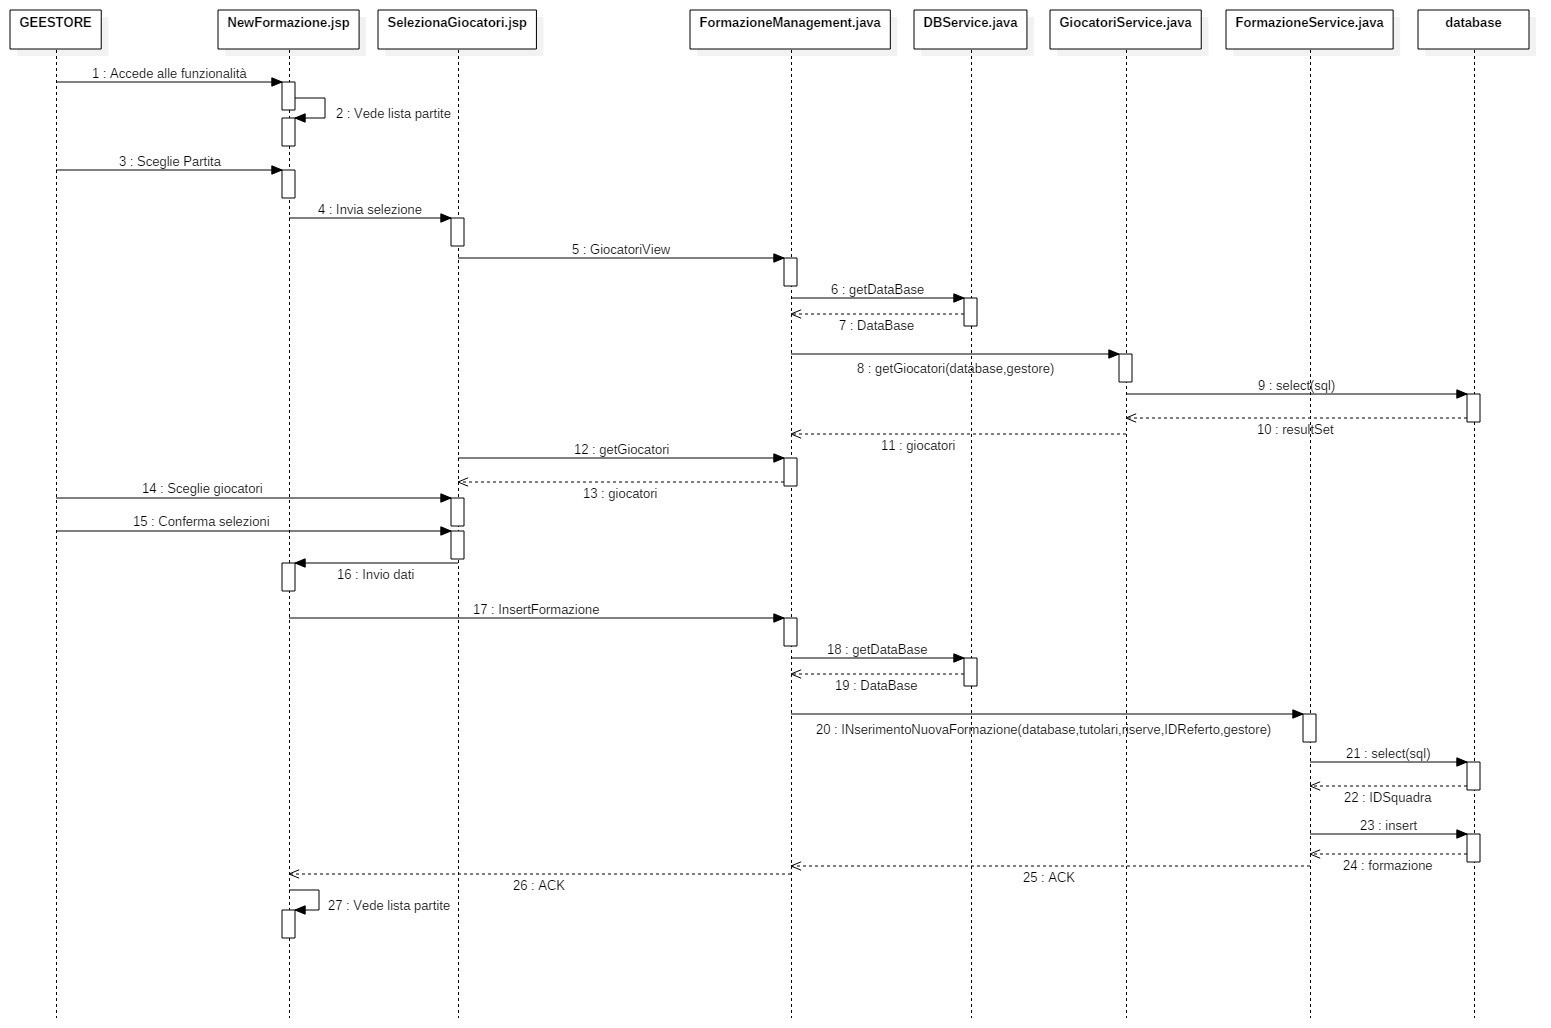
\includegraphics[width=1\textwidth]
	{immagini/sd-partita}
	
	\caption{Diagramma di sequenza della creazione della formazione di una squadra}
\end{figure}      % modello di design
%\appendix
%\input{capitoli/Dolor}
% *****************************************************************
% Materiale finale
%******************************************************************
%% !TEX encoding = UTF-8
% !TEX TS-program = pdflatex
% !TEX root = ../Tesi.tex
% !TEX spellcheck = it-IT

%*******************************************************
% Bibliografia
%*******************************************************
\cleardoublepage
\nocite{*}
\printbibliography
%% !TEX encoding = UTF-8
% !TEX TS-program = pdflatex
% !TEX root = ../Tesi.tex
% !TEX spellcheck = it-IT

%*******************************************************
% Dichiarazione
%*******************************************************
\cleardoublepage
\phantomsection
\pdfbookmark{Dichiarazione}{Dichiarazione}
\chapter*{Dichiarazione}
\thispagestyle{empty}

Lorem ipsum dolor sit amet, consectetuer adipiscing elit. Ut purus elit, vestibulum ut, placerat ac, adipiscing vitae, felis. Curabitur dictum gravida mauris. Nam arcu libero, nonummy eget, consectetuer id, vulputate a, magna. Donec vehicula augue eu neque.

Pellentesque habitant morbi tristique senectus et netus et malesuada fames ac turpis egestas. Mauris ut leo. Cras viverra metus rhoncus sem. Nulla et lectus vestibulum urna fringilla ultrices.

\bigskip
 
\noindent\textit{\myLocation, \MakeTextLowercase{\myTime}}

\smallskip

\begin{flushright}
    \begin{tabular}{m{5cm}}
        \\ \hline
        \centering\myName \\
    \end{tabular}
\end{flushright}

\end{document}